% Created 2023-08-24 Thu 19:19
% Intended LaTeX compiler: pdflatex
\documentclass[a4paper, 11pt, twoside]{book}
\usepackage[utf8]{inputenc}
\usepackage[T1]{fontenc}
\usepackage{graphicx}
\usepackage{longtable}
\usepackage{wrapfig}
\usepackage{rotating}
\usepackage[normalem]{ulem}
\usepackage{amsmath}
\usepackage{amssymb}
\usepackage{capt-of}
\usepackage{hyperref}
\usepackage[french]{babel}
\usepackage{color}
\usepackage{minted}
\usepackage{parskip}
\usepackage{tikz}
\usepackage{svg}
\usepackage{titletoc}
\usepackage{hyperref}
\hypersetup{colorlinks=true, linkcolor=blue, urlcolor=orange}
\newcommand{\N}{\mathbb{N}}
\newcommand{\Z}{\mathbb{Z}}
\newcommand{\D}{\mathbb{D}}
\newcommand{\Q}{\mathbb{Q}}
\newcommand{\R}{\mathbb{R}}
\newcommand{\intr}[4]{\left #1 #2\,;\,#3 \right #4}
\newcommand{\ceintr}[2]{\left[#1\,;\,#2\right]}
\newcommand{\disk}[3]{\left\lvert #1 - #2 \right\rvert \leq #3}
\usepackage[autostyle=true]{csquotes}
\usepackage[autostyle=true]{csquotes}
\usepackage[autostyle=true]{csquotes}
\usepackage[autostyle=true]{csquotes}
\usepackage[autostyle=true]{csquotes}
\usepackage[autostyle=true]{csquotes}
\usepackage[autostyle=true]{csquotes}
\usepackage[autostyle=true]{csquotes}
\usepackage[autostyle=true]{csquotes}
\usepackage[autostyle=true]{csquotes}
\usepackage[autostyle=true]{csquotes}
\usepackage[autostyle=true]{csquotes}
\usepackage[autostyle=true]{csquotes}
\usepackage[autostyle=true]{csquotes}
\usepackage[autostyle=true]{csquotes}
\usepackage[autostyle=true]{csquotes}
\usepackage[autostyle=true]{csquotes}
\usepackage[autostyle=true]{csquotes}
\usepackage[autostyle=true]{csquotes}
\usepackage[autostyle=true]{csquotes}
\usepackage[autostyle=true]{csquotes}
\usepackage[autostyle=true]{csquotes}
\usepackage[autostyle=true]{csquotes}
\usepackage[autostyle=true]{csquotes}
\usepackage[autostyle=true]{csquotes}
\usepackage[autostyle=true]{csquotes}
\usepackage[autostyle=true]{csquotes}
\usepackage[autostyle=true]{csquotes}
\usepackage[autostyle=true]{csquotes}
\usepackage[autostyle=true]{csquotes}
\usepackage[autostyle=true]{csquotes}
\usepackage[autostyle=true]{csquotes}
\usepackage[autostyle=true]{csquotes}
\usepackage[autostyle=true]{csquotes}
\usepackage[autostyle=true]{csquotes}
\usepackage[autostyle=true]{csquotes}
\usepackage[autostyle=true]{csquotes}
\usepackage[autostyle=true]{csquotes}
\usepackage[autostyle=true]{csquotes}
\author{Laurent Garnier}
\date{}
\title{Manipuler les nombres réels (avec solutions)}
\hypersetup{
 pdfauthor={Laurent Garnier},
 pdftitle={Manipuler les nombres réels (avec solutions)},
 pdfkeywords={},
 pdfsubject={},
 pdfcreator={Emacs 28.1 (Org mode 9.5.2)}, 
 pdflang={French}}
\begin{document}

\maketitle
\tableofcontents


\part{À qui s'adresse ce livre}
\label{sec:orge6d6875}
\begin{foreigndisplayquote}{english}
Mathematics is a language.\\

\href{https://en.wikipedia.org/wiki/Josiah\_Willard\_Gibbs}{Josiah Willard Gibbs}
\end{foreigndisplayquote}

Ce livre s'adresse initialement aux élèves de seconde du système
scolaire français. Mais il sera probablement très utile à un élève
de fin de collège qui voudrait assurer son entrée au lycée. Il sera
également très utile à un élève de première qui voudrait s'assurer
qu'il maîtrise bien les notions de la classe de seconde. Enfin un
quatrième public qui pourrait directement être visé est celui des
enseignants, profs particuliers ou encore tuteurs (professionnels ou
amateurs) qui souhaiteraient consulter des ressources utiles et
utilisables pour aider les lycéens.

De façon plus générale, même si je reprends exactement la structure
du programme officiel que vous pouvez consulter ici :
\url{https://eduscol.education.fr/document/24553/download}, il me semble
que ce livre pourrait être utile à quiconque souhaite approcher les
mathématiques de façon honnête, rigoureuse et avec un soucis de
compréhension. Tout en respectant le niveau du programme j'essaierai
dès que possible de prolonger la perspective.

Vous pouvez d'ores et déjà mettre en pratique de façon interactive
toutes les notions abordées grâce aux codes Python accessible sur
Google Colab à l'adresse communiquée dans la section concernée
lorsque vous aurez rempli ce petit formulaire :
\url{https://forms.gle/pT3GVr8PdNYCeVir7} (vous trouverez également les
corrections de tous les exercices du livre).

Si vous constatez une erreur que ça soit une erreur de calcul, une
faute de frappe ou quoique ce soit merci de me contacter à l'adresse
indiquée dans le formulaire afin de me la signaler et que je puisse
la corriger. Idem si vous avez des suggestions d'amélioration.


Bonne lecture.

\part{Contenus}
\label{sec:org4370264}
\startcontents[level-1]
\printcontents[level-1]{}{0}{\setcounter{tocdepth}{2}}
\begin{foreigndisplayquote}{english}
Mathematics has beauty and romance. It’s not a boring place to be,
the mathematical world. It’s an extraordinary place; it’s worth
spending time there.\\

\href{https://en.wikipedia.org/wiki/Marcus\_du\_Sautoy}{Marcus du Sautoy}
\end{foreigndisplayquote}

\chapter{Ensemble \(\R\) des nombres réels, droite numérique}
\label{sec:org4798595}
\startcontents[level-2]
\printcontents[level-2]{}{0}{\setcounter{tocdepth}{4}}

\begin{foreigndisplayquote}{french}
Tout l'univers repose sur l'ensemble des entiers naturels.\\
\href{https://fr.wikipedia.org/wiki/Pythagore}{Pythagore de Samos}
\end{foreigndisplayquote}


\section{Savez-vous compter sur vos doigts ?}
\label{sec:orge963e7c}

Savez-vous résoudre l'équation \(x - 1 = 0\) ? Je vous laisse
réfléchir et je vous donnerai la solution plus tard.

Imaginez que vous êtes en train de jouer à votre jeu vidéo
préféré. Il vous reste 3 points de vie, combien pouvez-vous en
perdre avant de mourir (dans le jeu) ? Idem, je vous laisse
réfléchir.

En général, lorsque vous entrez en seconde vous êtes âgé de 15 ans,
du coup combien d'années vous séparent de votre majorité ?

Ces trois questions traitent du même genre de problèmes, la
résolution des équations algébriques du premier degré impliquant
les nombres les plus simples que vous connaissez à savoir les
nombres entiers naturels. Pour la faire simple il s'agit des
nombres utiles pour compter le nombre de doigts que vous possédez,
le nombre d'enfants dans une famille et toutes les choses qu'on
peut dénombrer de zéro à l'infini.

On note l'ensemble des entiers naturels \[\N = \{0, 1, 2, 3,\dots
   \}\]


\begin{align*}
x - 1 &= 0 \Rightarrow x = 1\in\N\\
3 - x &= 0 \Rightarrow x = 3\in\N\\
15 + x&= 18\Rightarrow x = 3\in\N
\end{align*}

\section{Tout est relatif}
\label{sec:org5dbd163}

Mais ces nombres sont insuffisants pour exprimer des températures
par exemple dans une ville d'Europe du Nord comme Saint Pétersbourg
en Russie ou Oslo en Norvège. En fait, même en France
métropolitaine si vous allez en Savoie vous observerez des
températures négatives en hiver et positive en été. Le signe de ces
températures est \emph{relatif} à la position du zéro.

Les nombres entiers relatifs sont constitués des nombres entiers
naturels (les nombres positifs qu'on a vu précédemment) auquels on
ajoute leurs symétriques par rapport à zéro.

On les notes \(\Z = \{\dots, -2, -1, 0, 1, 2, \dots\}\).

Ce sont également ces nombres qu'on utilise dans un ascenseur pour
indiquer si on va au sous-sol (nombre négatif) ou aux étages
supérieurs (nombres positifs).

Dans le langage de programmation Python les nombres entiers
relatifs sont représentés par le type \texttt{int} pour \emph{integer} (qui
veut dire entier relatif en anglais).

\section{Les ordinateurs s'en contentent}
\label{sec:org393595a}

Mais ces nombres sont encore en nombre insuffisant pour exprimer
par exemple les unités monétaires. Quand vous achetez une baguette,
du carburant, des fournitures scolaires ou quoique ce soit ; la
plupart du temps vous utilisez des nombres à virgules qu'on appelle
les nombres décimaux.

Contrairement aux deux ensembles précédents, l'ensemble des nombres
décimaux ne peut pas être représenté de façon explicite avec des
points de suspension, il doit être définit en
\emph{compréhension}. Définir un ensemble en compréhension signifie que
vous devez expliquer la règle de construction.

On note [\D = \left$\backslash${ \dfrac{a}{10^n}$\backslash$,|$\backslash$,(a, n)\(\in\)\Z\textsuperscript{2\right}$\backslash$}$\backslash$]
l'ensemble des nombres décimaux avec le symbole \(|\) qui se lit
\emph{tel(s) que} et le symbole \(\in\) qui se lit \emph{appartient à}.

Commençons par la fin \((a, n)\in\Z^2\) signifie que \(a\) et
\(n\) sont tous les deux des entiers relatifs. Ainsi, les décimaux
sont les nombres fractionnaires dont le numérateur est un entier
relatif et le dénominateur une puissance de 10. Donnons quelques
exemples :
\begin{align*}
(a, n) &= (1, 2)\Rightarrow \dfrac{1}{10^2} = 0,01\\
(a, n) &= (3, 4)\Rightarrow \dfrac{3}{10^4} = 0,0003\\
(a, n) &= (2, -1)\Rightarrow \dfrac{2}{10^{-1}} = 20\\
(a, n) &= (3, 0)\Rightarrow \dfrac{3}{10^0} = 3\\
(a, n) &= (-1, 2)\Rightarrow \dfrac{-1}{10^2} = -0,01
\end{align*}

Dans la programmation Python on parle du type \texttt{float} pour
\emph{floating point number} ou nombre à virgule flottante en bon
français (puisque les anglo-saxons utilisent un point comme
séparateur décimal). En prenant \(n = 0\) on obtient tous les entiers
relatifs. Mais ce n'est pas suffisant pour décrire le réel (en
théorie, parce qu'en pratique les ordinateurs s'en contentent).

\section{Êtes-vous rationnels ?}
\label{sec:orgd8dac22}

Imaginez que vous avez un budget pour une semaine et que vous
souhaitiez allouer une part équitable pour chaque jour. Et bien
sachez que le nombre \(\dfrac{1}{7}\) n'est pas un décimal, pas plus
que le nombre \(\dfrac{1}{6}\). En effet si vous posez la division ou
que vous utilisez une machine (calculatrice, ordinateur, tablette
ou téléphone peu importe) vous verrez que \(\dfrac{1}{7} \simeq
   0,142857\dots\) et que cette séquence \(142857\dots\) se répètent à
l'infini. De même, de façon plus simple, si vous prenez
\(\dfrac{1}{6} \simeq 0,16\dots\) les 6 se répètent à l'infini.

Posons \(x = 0,16\dots 6\dots\) où les 6 se répètent à
l'infini. Multiplions par 100 ainsi on obtient \(100x = 16,6\dots
   6\dots\). Multiplions par 10 ainsi on obtient \(10x = 1,6\dots
   6\dots\). Faisons maintenant la soustraction \(90x = 15\) d'où \(x =
   \dfrac{15}{90} = \dfrac{3\times 5}{2\times 3\times 3\times 5} =
   \dfrac{1}{6}\). Le nombre \(\dfrac{1}{6}\) est bien un nombre qui sort
de la définition des décimaux et justifie une nouvelle classe de
nombres, les nombres rationnels (ratio en latin veut dire
quotient).

Les nombres rationnels sont notés \[\Q =
   \left\{\dfrac{a}{b}\,|\,(a,
   b)\in\Z\times\N^*\right\}\]

Ici le numérateur \(a\) est un entier relatif et le dénominateur \(b\)
est un entier naturel strictement positif parce qu'on ne peut pas
diviser par zéro.

Prouvons ce dernier résultat. Imaginez que l'on puisse trouver un
nombre entier \(a\) qui soit divisible par zéro. Alors il existerait
un entier \(q\) tel que \(a = 0\times q\). Le problème c'est que zéro
est un élément absorbant, tel le trou noir de la multiplication,
tout nombre multiplié par zéro donne zéro. La division par zéro n'a
donc pas de sens.

Donnons quelques exemples de nombre rationnels :

\begin{align*}
(a, b) &= (1, 2)\Rightarrow \dfrac{1}{2} = 0,5\in\D\\
(a, b) &= (8, 9)\Rightarrow \dfrac{8}{9} = 0,8\dots 8\dots\in\Q\\
(a, b) &= (3, 4)\Rightarrow \dfrac{3}{4} = 0,75\in\D\\
(a, b) &= (19, 11)\Rightarrow \dfrac{19}{11} = 1,72\dots \in\Q\\
(a, b) &= (2, 7)\Rightarrow \dfrac{2}{7} = 0,285714\dots \in\Q
\end{align*}

\section{Au-delà du réel}
\label{sec:org0c1dbcd}

Les nombres rationnels sont très intéressants mais ils restent
insuffisants pour capturer le réel. Imaginez que l'écran de votre
ordinateur portable soit un rectangle de longueur 16 cm pour une
largeur de 9 cm (c'est le fameux format 16/9). Alors pour calculer
la diagonale nous allons utiliser le théorème de Pythagore :
\begin{align*}
d^2 &= 16^2 + 9^2\\
d^2 &= 256 + 81\\
d^2 &= 337\\
d &= \sqrt{337} \simeq 18,36
\end{align*}

Tout d'abord le nombre 337 est un nombre premier (prouvez-le, c'est
un bon exercice). Et ensuite la racine carrée d'un nombre premier
ne peut pas s'écrire sous la forme d'un nombre rationnel.

Pour des raisons de concordance avec le programme de seconde je
vous propose de démontrer que \(\sqrt{2}\) n'est pas un nombre
rationnel et pour le résultat (plus général) énoncé précédemment,
je vous renvoie aux approfondissements (mais vous pouvez déjà
commencer à chercher).

Pour démontrer que \(\sqrt{2}\) n'est pas un nombre rationnel on va
utiliser plusieurs types de raisonnement. Tout d'abord nous allons
utiliser le raisonnement par l'absurde. Le raisonnement par
l'absurde repose sur un principe de la logique classique qui dit
qu'une affirmation est soit vraie soit fausse. En logique
mathématique on ne s'occupe que de ce genre d'affirmation donc nous
sommes dans un système \textbf{beaucoup} plus simple que la réalité. Du
coup, si le contraire de ce que je veux montrer est faux alors ce
que je veux montrer est vrai. Prenons un exemple concret un peu
simpliste, si ce n'est pas le matin alors c'est l'après-midi. Si
vous n'êtes pas majeur alors vous êtes mineur. Ce genre de logique
fonctionne bien avec les systèmes binaires.

Revenons à nos moutons, on veut montrer que \(\sqrt{2}\) n'est pas
rationnel donc on va supposons le contraire et montrer que ce
contraire est faux donc que notre affirmation sera vraie.

Supposons donc par l'absurde que \(\sqrt{2}\) soit rationnel donc
d'après la définition de \(\Q\) il devrait exister un entier
relatif \(a\) et un entier naturel strictement positif \(b\) tels que
\(\sqrt{2} = \frac{a}{b}\). Comme toute fraction peut se ramener
(après simplification) à une fraction irréductible on peut donc
considérer que \(a\) et \(b\) n'ont pas de diviseurs communs et que la
fraction est irréductible. Dire que \(a\) et \(b\) n'ont pas de
diviseurs communs revient à dire que leur pgcd vaut un c'est-à-dire
\(pgcd(a, b) = 1\). Le PGCD est le Plus Grand Commun Diviseur. Bon on
devrait l'appeler le PGDC parce qu'en français on dit diviseur
commun car l'adjectif vient après le nom mais en anglais ils disent
\emph{greatest common divisor} et bien souvent les gens importent les
concepts anglophones en oubliant les règles du français c'est pour
ça que sur certaines calculatrices et logiciels vous pouvez voir
GCD ou gcd.

Faisons un bref récapitulatif :
\begin{itemize}
\item Objectif : Montrer que \(\sqrt{2}\) n'est pas rationnel
\item Méthode : Raisonnement par l'absurde, on pose \(\sqrt{2} =
     \frac{a}{b}\) et avec \(pgcd(a, b) = 1\)
\end{itemize}

Du coup, on va élever au carré ce qui nous donne \(2 =
   \frac{a^2}{b^2}\) et qu'on peut mettre sous la forme \(a^2 = 2b^2\).

On peut classer les nombres entiers en deux catégories :
\begin{enumerate}
\item Les nombres pairs de la forme \(p = 2n\) où \(n\) est un entier.
\item Les nombres impairs de la forme \(i = 2n + 1\) où \(n\) est un
entier.
\end{enumerate}

On en déduit que le nombre \(a^2 = 2b^2\) appartient à la première
catégorie avec \(n = b^2\).

Désormais on va avoir besoin d'un résultat intermédiaire qui va
faire intervenir un autre type de raisonnement (pour voir les
différents types de raisonnement consulter la playlist éponyme en
cliquant \href{https://www.youtube.com/watch?v=R\_L4NEgIxPM\&list=PLwWStLtwGECb-3dJmBXOYc8oQw1mRsrep\&pp=iAQB}{ici}).

Voici le résultat intermédiaire qu'on veut montrer : \emph{si le carré
d'un nombre est pair alors le nombre initial est aussi pair}.

On va formaliser cette affirmation :
\begin{itemize}
\item A = "le carré d'un nombre est pair"
\item B = "le nombre initial est pair"
\item \(P = A\Rightarrow B\)
\end{itemize}

Le nouveau type de raisonnement qu'on va utiliser s'appelle le
raisonnement par contraposée.

Prenons un exemple concret fictif (et simpliste). Imaginez que
chaque fois qu'il pleut je prenne mon parapluie (sans \textbf{aucune}
exception). Si vous me croisez \textbf{sans} parapluie alors vous en
déduirez qu'il ne pleut pas. C'est une proposition logiquement
équivalente à la première formulation.

\begin{enumerate}
\item A = "Il pleut"
\item B = "Je prend mon parapluie"
\item \(P = A\Rightarrow B\)
\item non B = "Je n'ai pas de parapluie"
\item non A = "Il ne pleut pas"
\item \(CP(P) = non(B)\Rightarrow non(A)\)
\end{enumerate}

Revenons à nos nombres entiers. La contraposée de : "Si le carré
d'un nombre est pair alors le nombre initial est aussi pair." est
"Si le nombre initial est impair alors son carré aussi."

Décomposons :
\begin{align*}
 A &= \text{"le carré d'un nombre est pair"}\\
 B &= \text{"le nombre initial est pair"}\\
 P &= \text{A\Rightarrow B}\\
 non(B) &= \text{"le nombre initial est impair"}\\
 non(A) &= \text{"le carré est impair"}\\
 CP(P) &= non(B)\Rightarrow non(A)
 \end{align*}

Ce raisonnement nous permet de ramener la proposition à montrer à
une proposition plus simple et qu'on peut montrer directement.

Si le nombre initial est impair alors il est de la forme \(i = 2n +
   1\). Il vient que son carré satisfait :
\begin{align*}
i^2 &= (2n + 1)^2\\
i^2 &= (2n)^2 + 2\times 2n\times 1 + 1^2\\
i^2 &= 2(2n^2 + 2n) + 1
\end{align*}

On a bien obtenu un nombre impair. Par équivalence logique la
proposition initiale est vraie.

Faisons un bilan d'étape.
\begin{enumerate}
\item Objectif final : Montrer que \(\sqrt{2}\) n'est pas rationnel
\item Méthode : Raisonnement par l'absurde, on pose \(\sqrt{2} =
     \frac{a}{b}\) et avec \(pgcd(a, b) = 1\)
\item Objectif intermédiaire : \(a^2 = 2b^2\) est pair donc \(a\) est pair.
\item Méthode pour l'objectif intermédiaire : raisonnement par
contraposée, si \(a\) est impair alors \(a^2\) aussi
\end{enumerate}

À ce stade nous avons bien montré que \(a^2 = 2b^2\) entraîne que
\(a = 2n\). De cette nouvelle écriture on tire \(a^2 = 4n^2\) et on
peut établir une nouvelle égalité \(2b^2 = 4n^2\) qui donne \(b^2 =
   2n^2\). Par conséquent, en utilisant notre résultat intermédiaire,
on constate que \(b\) est aussi pair.

Mais si \(a\) et \(b\) sont pairs alors ils sont divisibles par deux ce
qui contredit \(pgcd(a, b) = 1\). Ce résultat est absurde donc
l'hypothèse initiale aussi et finalement \(\sqrt{2}\) n'est pas un
rationnel. CQFD

Bravo à vous si vous avez tout compris. Pour les autres,
rassurez-vous, c'est normal que ça chauffe dans votre tête. Vous
pouvez déjà revoir cette démonstration en vidéo ici :
\url{https://youtu.be/R\_L4NEgIxPM}

Le raisonnement par l'absurde consiste à partir d'une hypothèse
contraire à celle qu'on souhaite montrer et ensuite à enchaîner des
déductions logiques parfaitement valides jusqu'à aboutir à une
contradiction. La chaîne de déductions peut parfois s'avérer (très)
longue et impliquer des résultats intermédiaires nécessitant à leur
tour (éventuellement) d'autres types de raisonnement.

Dans certains ouvrages, certaines personnes préfèrent admettre les
résultats intermédiaires. Dans l'absolu il serait impossible de
tout démontrer parce qu'on ne pourrait jamais avancer. Néanmoins il
est utile de garder à l'esprit qu'en mathématiques le but du jeu
est de démontrer les affirmations sans jamais les prendre pour
argent comptant.

Finalement, puisque \(\sqrt{2}\) n'est pas un nombre rationnel il
doit bien appartenir à un ensemble de nombre et cet ensemble est
l'ensemble des nombres réels et on le note \(\R\).

Nous avons ainsi la chaîne d'inclusions ensemblistes :

\[\N\subset\Z\subset\D\subset\Q\subset\R\]

Cet ensemble de nombres correspond à l'infinité des points sur une
droite et c'est pour cette raison qu'on représentera souvent les
nombres réels par une droite graduée qu'on appellera la droite des
réels avec 0 au milieu et qui se prolonge vers \(+\infty\) à droite
et \(-\infty\) à gauche.

\[-\infty --\left(-\frac{5}{3}\right)-(-\sqrt{2})--(-1)--(0)--(+1)--(+\Phi)--(+\pi)-->+\infty\]

\section{Raisonnement par contraposition}
\label{sec:org298f45f}

Revenons un petit instant sur la mécanique du raisonnement par
contraposée. Pour cela on va décortiquer l'implication logique.

\begin{align*}
A &=\,"x > 2"\\
B &=\,"2x > 4"\\
P &=\,A\Rightarrow B\\
\neg B &=\, "2x \leq 4"\\
\neg A &=\, "x \leq 2"\\
CP(P) &=\,(\neg B)\Rightarrow(\neg A)
\end{align*}

Le symbole \(\neg\) est la négation logique.

\section{Exercice}
\label{sec:org02c154b}
Reprennez la même mécanique présentée ci-dessus avec cette fois \(A
    = "x < -1"\) et \(B = "-3x > 3"\).

Voir solution \ref{sec:org9049a7b}

\section{Exercice Python}
\label{sec:orga38a814}
\begin{enumerate}
\item Écrire une fonction Python \texttt{imply} qui prend deux arguments en
entrée et renvoie la phrase logique "A implique B" avec A et B
remplacés par leurs valeurs.
Par exemple : \texttt{imply("x > 1", "x**2 > 1")}
renverra \texttt{"'x > 1'implique 'x**2 > 1'"}
\item Écrire une autre fonction Python \texttt{contrapose} qui prend deux
arguments A et B et qui renvoie la contraposée de "A implique
B". Donc la fonction devra renvoyer "non B implique non
A". Votre programme écrira littéralement "non" suivie de la
valeur de la proposition A (ou B) parce que vous ne pouvez pas
(en tout cas je ne sais pas) modifier logiquement le contenu
d'une chaîne de caractères avec Python.
\end{enumerate}

Voir solutions \ref{sec:org49e8be4}
\stopcontents[level-2]

\chapter{Intervalles de \(\R\). Notations \(+\infty\) et \(-\infty\)}
\label{sec:org7096b61}
\startcontents[level-2]
\printcontents[level-2]{}{0}{\setcounter{tocdepth}{4}}

\begin{foreigndisplayquote}{english}
One of the big misapprehensions about mathematics that we
perpetrate in our classrooms is that the teacher always seems to
know the answer to any problem that is discussed.\\
\href{https://en.wikipedia.org/wiki/Leon\_Henkin}{Leon Henkin}
\end{foreigndisplayquote}


\section{Introduction de la notion d'intervalle}
\label{sec:org1fe44cf}

Jusqu'à présent nous avons traité essentiellement des égalités (une
équation est une égalité). Mais dans de nombreux cas il est
intéressant et utile de traiter des inégalités. Donnons quelques
exemples issus du monde réel de la vie de tous les jours :
\begin{enumerate}
\item Il faut être âgé de plus de 14 ans pour conduire un véhicule de
type mobilette ou scooter.
\item Il faut être âgé entre 12 et 25 ans pour bénéficier du tarif
jeune à la SNCF.
\item Les films pornographiques sont interdits aux mineurs donc aux
gens qui ont un âge inférieur à 18 ans.
\item En boxe anglaise la catégorie de poids pailles concerne les gens
dont le poids est inférieur à 47,128 kg (soit 105 livres, source :
\url{https://fr.wikipedia.org/wiki/Boxe\_anglaise} )
\item En France, seuls les gens qui ont moins de 10 777€ par an sont
exonérés d'impôt (0\%), ensuite de 10 778 à 27 478 c'est 11\%,
puis 30\% de 27 479 à 78 570, puis 41\% de 78 571 à 168 994 et
enfin 45\% pour ceux qui ont plus de 168 994 (source :
\url{https://www.service-public.fr/particuliers/vosdroits/F1419} )
\item La limite autorisée du taux d'alcool dans le sang par la loi en
2023 est de 0,5 g/L soit en équivalent 0,25 mg par litre d'air
expiré (source :
\url{https://www.legipermis.com/infractions/alcool-permis-conduire.html}
)
\item L'IMC (Indice de Masse Corporelle) permet d'établir des
catégories pour mesurer l'obésité avec par exemple le début de la
surcharge pondérale (surpoids) à partir de 25 kg/m\textsuperscript{2} (source :
\url{https://fr.wikipedia.org/wiki/Indice\_de\_masse\_corporelle} )
\end{enumerate}

Traduisons ces exemples concrets en inégalités mathématiques. Dans
chaque cas on utilisera la lettre \(x\) pour désigner la variable
inconnue.

\begin{enumerate}
\item \(x \geq 14\)
\item \(12 \leq x \leq 25\)
\item \(0 < x < 18\)
\item \(0 < x < 47,128\)
\item \(0 \leq x \leq 10 777\)
\item \(0 \leq x < 0,5\)
\item \(x \geq 25\)
\end{enumerate}

Ces inégalités peuvent être représentées graphiquement. On peut les
interpréter comme des zones délimitées par des bornes inférieures
et supérieures. Lorsqu'il n'y a qu'une seule borne apparente alors
ça veut dire que l'autre est du type \(\infty\) avec le signe
adéquat.

Traduisons ces inégalités en intervalles :

\begin{enumerate}
\item \(x \geq 14 \iff x\in \intr{[}{14}{+\infty}{[}\) on parle d'intervalle fermé.
\item \(12 \leq x \leq 25\iff x\in \intr{[}{12}{25}{]}\) on parle d'intervalle fermé.
\item \(0 < x < 18\iff x\in \intr{]}{0}{18}{[}\) on parle d'intervalle ouvert.
\item \(0 < x < 47,128\iff x\in \intr{]}{0}{47,128}{[}\) on parle d'intervalle
ouvert.
\item \(0\leq x \leq 10 777\iff x\in \intr{[}{0}{10777}{]}\) on parle d'intervalle
fermé.
\item \(0 \leq x < 0,5\iff x\in [0\,;\,0,5[\) on parle d'intervalle ouvert à droite
\item \(x \geq 25\iff \in \intr{[}{25}{+\infty}{[}\) on parle d'intervalle fermé.
\end{enumerate}


Alors ici il s'agissait de modéliser à partir du monde réel donc il
y a des bornes implicites qui sont apparues :
\begin{enumerate}
\item Jusqu'à présent personne n'a dépassé le record de longévité de
Jeanne Calmant qui a vécu 122 ans. Mais comme on ne peut pas
prédire l'avenir alors j'ai décidé de mettre la borne \(+\infty\)
même si c'est une borne théorique. Néanmoins, certains ont
prédit \href{https://amzn.to/3OKi2os}{la mort de la mort} (c'est le titre d'un livre de Laurent
Alexandre).
\item Ici les bornes étaient claires.
\item Là j'ai considéré que l'âge zéro n'est jamais atteint puisque
dès l'instant où l'on naît le temps s'écoule. Mais au regard de
l'exemple j'aurais même pu mettre une borne inférieure plus
grande.
\item Dans cet exemple c'est la même idée, personne n'a un poids de
zéro et encore moins quand on pratique la boxe anglaise.
\item Pour les revenus c'est malheureusement différent, il est hélas
possible d'avoir zéro revenu. Et pour information, 10 777 par an
ça fait moins de 900€ par mois (environ 898,08).
\item Les gens qui ne boivent pas d'alcool peuvent avoir un taux de
zéro gramme dans le sang.
\item Comme pour l'âge, le poids maximal n'est pas figé, d'ailleurs on
devrait parler de masse parce que le poids est une force qui
dépend du champ gravitationnel (la pesanteur) et donc il peut
changer en fonction de l'endroit dans l'espace.
\end{enumerate}

Traduisons ces intervalles en représentations graphiques :

\begin{enumerate}
\item \(x \geq 14 \iff x\in [14; +\infty [\) on parle d'intervalle
fermé. 14 est compris dans l'intervalle.

\[[14--------------------->+\infty\]

\item \(12 \leq x \leq 25\iff x\in [12; 25]\) on parle d'intervalle
fermé. 12 et 25 sont inclus dans l'intervalle.

\[[12-----25]\]

\item \(0 < x < 18\iff x\in ]0; 18[\) on parle d'intervalle ouvert.
0 et 18 sont exclus de l'intervalle.

\[0]-----------[18\]

\item \(0 < x < 47,128\iff x\in ]0; 47,128[\) on parle d'intervalle
ouvert. \(0\) et \(47,128\) sont exclus de l'intervalle.

\[0]----------------[47,128\]

\item \(0\leq x \leq 10 777\iff x\in [0; 10777]\) on parle d'intervalle
fermé. 0 et 10777 sont inclus dans l'intervalle.

\[[0---------------------------10777]\]

\item \(0 \leq x < 0,5\iff x\in [0; 0,5[\) on parle d'intervalle ouvert
à droite. \(0\) est inclu mais \(0,5\) est exclu de l'intervalle.

\[[0---[0,5\]

\item \(x \geq 25\iff \in [25; +\infty[\) on parle d'intervalle
fermé. 25 est inclu dans l'intervalle.

\[[25------------------------------>+\infty\]
\end{enumerate}


Ces exemples concrets avaient pour but de vous montrer pourquoi ce
principe de représentation d'ensembles de nombres réels ordonnés
peut avoir un intérêt et une utilité.

Les différents types d'intervalles de \(\R\) sont les
suivants :
\begin{enumerate}
\item Les intervalles ouverts à bornes finies \(]a ; b[\).
\[a]-----[b\]
\item Les intervalles ouverts à gauche à bornes finies \(]a ; b]\) (on
peut aussi les appeler fermés à droite).
\[a]-------b]\]
\item Les intervalles ouverts à droite à bornes finies \([a ; b[\) (on
peut aussi les appeler fermés à gauche).
\[[a--------[b\]
\item Les intervalles ouverts à borne infinie à gauche \(]-\infty ;
      b[\).
\[-\infty ]-----------------------[b\]
\item Les intervalles ouverts à borne infinie à droite \(]a ;
      +\infty[\).
\[a]-------------------------->+\infty\]
\item Les intervalles fermés à borne infinie à gauche \(]-\infty ; b]\).
\[-\infty ]-----------------------b]\]
\item Les intervalles fermés à borne infinie à droite \([a ; +\infty[\).
\[[a--------------------------->+\infty\]
\item Les intervalles fermés à bornes finies \([a ; b]\).
\[[a--------b]\]
\item L'intervalle ouvert \textbf{ET} fermé de l'ensemble des réels tout
entier \[\R\,=\,]-\infty ; +\infty[\]
\[-\infty --------------------------> +\infty\]
\end{enumerate}

Il est important de rappeler qu'un intervalle est forcément ordonné
donc la borne supérieure (à droite) est forcément plus grande que
la borne inférieure (à gauche) sinon ça n'a strictement aucun
sens.

Donnons quelques exemples :
\begin{align*}
\frac{1}{2} &\in ]0 ; 1[ \\
1 &\in ]0 ; 1] \\
-\frac{1}{2} &\in [-0,5 ; 0[\\
-1 &\in ]-\infty ; 1[\\
\frac{2}{3} &\in ]0 ; +\infty[ \\
\pi &\in [3 ; +\infty[ \\
\Phi = \frac{1 + \sqrt{5}}{2} &\in [1 ; 2] \\
\tau = 2\pi &\in \R
\end{align*}

On peut remarquer que l'ensemble des nombres entiers naturels est
inclus dans l'ensemble des nombres réels positifs :
\[\N\subset \R_{+} = [0; +\infty[\]

Par contre entre deux entiers naturels il y a une infinité de réels
et pour les représenter on utilise un intervalle.

Prenons par exemple les deux plus petits entiers naturels zéro et
un. On peut construire un intervalle \(I_0 = [0 ; 1]\) qui les contient
tous les deux. Le centre de cet intervalle \(I_0\) est un nombre décimal
\(\frac{1}{2} = 0,5\). Construisons un nouvel interval \(I_1 = [0;
   0,5]\). Le centre de cet intervalle \(I_1\) est un nombre décimal
\(\dfrac{1}{4} = 0,25\). On pourrait continuer ainsi à l'infini en
construisant des intervalles de la forme \[I_n = \left[0 ;
   \dfrac{1}{2^n}\right]\]

Mais si au lieu de prendre le centre on prenait le premier tiers ?
Et bien cette fois on aurait une borne supérieure qui serait un
nombre rationnel. \[J_n = \left[0 ; \dfrac{1}{3^n}\right]\]

Et si au lieu de prendre le tiers on divisait par le nombre \(\pi\) ?
Et bien cette fois on aurait une borne supérieure qui serait un
nombre réel. \[K_n = \left[0 ; \dfrac{1}{\pi^n}\right]\]

Bon dans ce dernier cas j'ai un peu triché parce que \(\pi\) est déjà
un réel alors que pours les \(I_n\) et les \(J_n\) on a pu faire la
construction uniquement en utilisant des entiers naturels.

Prenons un peu la mesure de ce que nous faisons. L'intervalle \([0 ;
   1]\) a pour longueur \(1\) de même que l'intervalle \([1 ; 2]\). Mais
qu'en est-il de l'intervalle \([-1 ; 0]\) ? \([-1 ; 1]\) ? Et de façon
générale, comment mesure-t-on la longueur d'un intervalle ?

C'est très simple, un intervalle étant un ensemble ordonné, on
mesure sa longueur en soustrayant la borne inférieure à la borne
supérieure (que l'intervalle soit ouvert ou fermé).

Il y a donc deux cas de figure :
\begin{enumerate}
\item Les bornes \(a\) et \(b\) sont finies et dans ce cas c'est juste une
soustraction normale \(|I| = |b - a|\).
\item Au moins l'une des bornes est infinie et dans ce cas \(|I| =
      +\infty\).
\end{enumerate}

Voici quelques exemples :
\begin{align*}
\lvert ]-3 ; 3] \rvert &= 3 - (-3) = 3 + 3 = 6\\
\lvert [-5 ; 4] \rvert &= 5 - (-4) = 5 + 4 = 9\\
\lvert ]-\infty ; 23] \rvert &= +\infty\\
\lvert [7 ; +\infty[ \rvert &= +\infty\\
\lvert ]-\infty ; +\infty] \rvert &= +\infty
\end{align*}

La longueur d'un intervalle est aussi appelée son amplitude. Par
exemple le nombre \(\pi\) appartient à l'intervalle \([3,14 ; 3,15]\)
qui a pour amplitude \(10^{-2} = 0,01\). Dit autrement, le nombre
\(\pi\) est compris entre \(3,14\) et \(3,15\) à \(10^{-2}\) près.

\section{Exercice}
\label{sec:org3ebd799}
Faisons un petit exercice. Pour les nombres suivants trouver des
intervalles d'amplitude \(10^{-1}\) puis \(10^{-2}\) et enfin \(10^{-3}\)
auquels ils appartiennent :
\begin{enumerate}
\item \(\dfrac{1}{3}\)
\item \(\sqrt{2}\)
\item \(\Phi = \dfrac{1 + \sqrt{5}}{2}\)
\item \(\pi\)
\item \(\tau = 2\pi\)
\end{enumerate}

Jouez le jeu en cherchant par vous même vous progresserez alors que
si vous regardez la solution directement il vous progression sera
nulle.

Voir solutions \ref{sec:org0af5bba}

\section{Exercice}
\label{sec:orgddaeb73}
\begin{enumerate}
\item À l'aide d'une machine calculez les 5 premières décimales du nombre d'or
\[\Phi = \dfrac{1 + \sqrt{5}}{2}\]
\item Considérez la suite de nombres :

\begin{align*}
 F_1 = 1&& F_2 = 1&& F_3 = 2&& F_4 = 3\\
 F_5 = 5&& F_6 = 8&& F_7 = 13&& F_8 = 21\\
 F_9 = 34&& F_{10} = 55&& F_{11} = 89&&\dots
\end{align*}

Calculez les 5 termes suivants.
\item Établir la règle de construction de la suite.
\item Calculer les quotients successifs en prenant comme numérateur le
suivant et comme dénominateur le prédécesseur ainsi
\(\dfrac{1}{1}, \dfrac{2}{1}, \dfrac{3}{2},\dots\).
\item La suite de nombre de la question 2 est connue sous le nom de
\href{https://fr.wikipedia.org/wiki/Suite\_de\_Fibonacci}{suite de Fibonacci} (mathématicien italien du XIIème siècle qui a
appris l'usage des chiffres indo-arabes grâce à son père qui
commerçait avec des marchands arabes près d'Alger). Combien de
termes de cette suite faut-il calculer pour approcher le nombre
d'or à \(10^{-5}\) près ? Vous donnerez les intervalles successifs.
\end{enumerate}


Voir solutions \ref{sec:org5140565}

\section{Petit jeu}
\label{sec:orgb808075}
Faisons un petit jeu. Voici une série de nombres particuliers :
\begin{enumerate}
\item \(u = 0,1\dots\) avec une infinité de 1
\item \(v = 0,12\dots\) avec une infinité de 12
\item \(w = 0,123\dots\) avec une infinité de 123
\item \(x = 0,1234\dots\) avec une infinité de 1234
\item \(y = 0,12345\dots\) avec une infinité de 12345
\end{enumerate}

Pour chacun de ces nombres on va donner un intervalle d'amplitude
égale à la position de la dernière décimale distincte (donc 0,1
pour \(u\), 0,01 pour \(v\), 0,001 pour \(w\) et ainsi de suite) et
centré en ce nombre. Puis on va déterminer la fraction qui le
définit.

Voir solutions \ref{sec:org4a65d03}
\stopcontents[level-2]

\chapter{Notation |a|. Distance entre deux nombres réels}
\label{sec:org709c246}
\startcontents[level-2]
\printcontents[level-2]{}{0}{\setcounter{tocdepth}{4}}

\begin{foreigndisplayquote}{french}
Les maths, ça prend le relais dans les situations où l’intelligence
habituelle est en panne. Les chaussures sont un instrument pour
marcher, les maths sont un instrument pour penser. On peut marcher
sans chaussures, mais on va moins loin.\\
\href{https://fr.wikipedia.org/wiki/Jean-Marie\_Souriau}{Jean-Marie Souriau}
\end{foreigndisplayquote}

\section{Introduction de la notion de distance}
\label{sec:orga191266}

Quelle est la distance entre 0 et 1 ? Facile, c'est 1 ! Quelle est
la distance entre \(\frac{1}{2}\) et \(\frac{1}{3}\) ? Là déjà c'est
plus tout à fait la même histoire. Il va falloir réfléchir un peu à
la façon de procéder. Prenons d'abord encore quelques exemples plus
simples. Quelle est la distance entre \(-1\) et 0 ? Facile, c'est 1 !
Quelle est la distance entre \(-1\) et \(1\) ? Vous avez trouvé ? Oui
c'est 2. Quelle la distance entre \(\frac{1}{2}\) et \(1\) ? Oui c'est
\(0,5\).

Bon, avant de donner la règle générale, ramenons les choses à un
problème plus simple. Quelle est la distance d'un nombre par
rapport à zéro ? Prenons le nombre \(5\) par exemple, sa distance à
zéro est tout simplement 5. Est-ce le seul nombre à cette distance
de zéro ? Ben non puisque le nombre \(-5\) est aussi à une distance 5
par rapport à zéro. En fait, chaque nombre positif est exactement à
une distance à zéro égale à lui-même et son opposé est aussi à la
même distance mais de l'autre côté. Faisons un schéma :

\[-(-5)-(-4)-(-3)-(-2)-(-1)-0-(+1)-(+2)-(+3)-(+4)-(+5)->\]

On notera \(|a|\) la distance du nombre \(a\) par rapport à zéro. On
l'appelle aussi la valeur absolue de \(a\).

Donnons quelques exemples :

\begin{align*}
\lvert -1 \rvert = 1& = \lvert 1 \rvert \\
\lvert -2 \rvert = 2& = \lvert 2 \rvert \\
\lvert -3 \rvert = 3& = \lvert 3 \rvert \\
\lvert -\sqrt{2} \rvert = \sqrt{2}& = \lvert \sqrt{2} \rvert \\
\lvert -\pi \rvert = \pi& = \lvert \pi \rvert
\end{align*}

Une façon simple de décrire la chose est de dire que la valeur
absolue d'un nombre c'est le nombre sans le signe.

On peut désormais définir proprement la valeur absolue d'un nombre
réel \(a\) : \[\lvert a \rvert = s(a)a\] avec \(s(a) = 1\) si \(a\in[0 ;
   +\infty[\) et \(s(a) = -1\) si \(a\in ]-\infty ; 0]\). Autrement dit la
fonction \(s\) attribue le signe d'un nombre. Si un nombre est
positif il est égal à sa valeur absolue sinon il est égal à son
opposé.

Par exemple \(\lvert 9 \rvert = 9\) et \(\lvert -7\rvert = -(-7) = 7\).

Mais revenons à notre problème initial. Et concrétisons-le un peu
d'abord. Si vous parcourez 5 km vers l'Est puis que vous parcourez
3 km vers l'Ouest alors vous vous retrouverez 2 km à l'Est de votre
position initiale. Mais vous aurez parcouru 8 km (5 + 3). Si on
considère votre position initiale comme le zéro et le sens vers
l'Est comme le sens positif et le sens vers l'Ouest comme le sens
négatif alors le calcul de la position finale devient \(5 - 3 =
   2\). Pour fixer les idées on va nommer les différents points. Posons
\(O\) l'origine de cet axe horizontal (Est-Ouest). Soit \(A\) le point
d'abscisse \(x_A = 5\) et \(B\) le point d'abscisse \(x_B = -3\). La
distance entre \(A\) et \(B\) s'obtient en faisant le calcul \(x_A - x_B
   = 5 - (-3) = 5 + 3 = 8\). Mais pourquoi devrions-nous commencer par
\(A\) ? Une distance n'a pas d'orientation. Que vous fassiez 100 km à
l'Est ou 100 km à l'Ouest dans les deux cas la distance parcourue
sera de 100 km. Donc on devrait retrouver le même résultat que le
considère le point \(A\) ou le point \(B\) comme point de
départ. Pourtant \(x_B - x_A = -3 - 5 = -8\)\ldots{} aïe ! On dirait que
ça coince\ldots{} Ben pas tant que ça si on se souvient que la valeur
absolue c'est le nombre sans le signe. OK mais pourquoi utiliser la
valeur absolue ? Qu'est-ce qui justifie son usage ici ? Pour aller
du point \(B\) au point \(A\) il y a trois possibilités :
\begin{enumerate}
\item Soit le point \(O\) est avant le point \(B\) qui lui-même est avant
le point \(A\) et dans ce cas il faut d'abord parcourir la
distance de \(O\) à \(A\) puis retrancher celle de \(B\) à \(O\). Donc
si on schématise on obtient un axe horizontal orienté comme ceci
\[---O---B-----A---->\]
Ici on a \(AB = OA - OB = |x_A| - |x_B| = x_A - x_B = d_{AB}\)
\item Soit le point \(B\) est avant \(O\) et dans ce cas vous devez
d'abord parcourir la distance de \(B\) à \(O\) puis celle de \(A\) à
\(O\). Donc si on schématise on obtient un axe horizontal orienté
dans ce sens \[------B---O-----A------->\]
Ici on a \(AB = BO + OA = \lvert x_B \rvert + \lvert x_A \rvert =
      -x_B + x_A = x_A - x_B = d_{AB}\)
\item Soit le point \(O\) est après le point \(A\) qui lui-même est après
le point \(B\). Donc si on schématise on obtient un axe horizontal
orienté de cette façon \[--B----A---O---->\]
Ici on a \(AB = BO - OA = |x_B| - |x_A| = -x_B - (-x_A) = x_A -
      x_B = d_{AB}\)
\end{enumerate}


Dans les 3 cas on aboutit au même calcul final la différence entre
le grand moins le petit.


À l'issue de cette concrétisation on pourrait se dire que pour
calculer la distance entre deux nombres réels il suffit de calculer
la valeur absolue de leur différence. Spoiler alert, c'est
exactement ça ! La distance entre les nombres réels \(a\) et \(b\)
vaut :
\[d(a; b) = \lvert a - b \rvert = \lvert b - a \rvert = max(a ;
   b) - min(a ; b)\]


Donnons quelques exemples :

\begin{align*}
(a; b) = (1; 2) &\Rightarrow d(1; 2) = \lvert 1 - 2 \rvert = \lvert -1\rvert = 1\\
(a; b) = (2; 1) &\Rightarrow d(2; 1) = \lvert 2 - 1 \rvert = \lvert 1\rvert = 1\\
(a; b) = (1,5; 2,7) &\Rightarrow d(1,5; 2,7) = \lvert 1,5 - 2,7 \rvert = \lvert -1,2\rvert = 1,2\\
(a; b) = \left(\frac{1}{2}; \frac{1}{3}\right) &\Rightarrow d\left(\frac{1}{2}; \frac{1}{3}\right) = \lvert \frac{1}{2} - \frac{1}{3} \rvert = \lvert \frac{3}{6} - \frac{2}{6}\rvert = \frac{1}{6}\\
(a; b) = (\sqrt{2}; \pi) &\Rightarrow d(\sqrt{2}; \pi) = \lvert \sqrt{2} - \pi \rvert = \pi - \sqrt{2}
\end{align*}

Afin de revenir sur ce qu'on a déjà vu on peut aussi voir le
distance entre deux réels \(a\) et \(b\) comme l'amplitude de
l'intervalle entre le maximum et le minimum des deux. Ainsi :
\[d(a ; b) = |[min(a ; b) ; max(a ; b)]| = max(a ; b) - min(a ; b)\]

\section{Exercice}
\label{sec:org44a8f75}
Pour vous entraîner voici un exercice.

\begin{enumerate}
\item Calculer la distance entre \(\pi\) et \(\Phi = \frac{1 +
       \sqrt{5}}{2}\). Vous donnerez une approximation à 3 chiffres
après la virgule.
\item Calculer la distance \(\frac{1}{4}\) et \(\frac{1}{3}\). Vous
donnerez une approximation à 3 chiffres près.
\item Calculer la distance \(\frac{1}{7}\) et \(\frac{1}{8}\). Vous
donnerez une approximation à 6 chiffres.
\item Calculer la distance entre \(\Phi\) et \(\sqrt{2}\). Vous donnerez
une approximation à 2 chiffres.
\item Calculer la distance entre \(\Phi\) et \(\sqrt{3}\). Vous donnerez
une approximation à 5 chiffres.
\end{enumerate}

Voir solutions \ref{sec:org8dea703}

\section{Exercice}
\label{sec:orgf3fa79d}
Faisons un exercice intéressant. Renversons le point de vue. Au
lieu de calculer la distance entre deux points, cherchons les
points situés à une distance choisie par rapport à un point fixe.

\begin{enumerate}
\item Calculer les nombres à une distance 1 de 1.
\item Calculer les nombres à une distance \(0,5\) de \(-1\).
\item Calculer les nombres à une distance \(\frac{1}{3}\) de
\(\dfrac{1}{4}\).
\item Calculer les nombres à une distance \(\sqrt{2}\) de 1.
\item Calculer les nombres à une distance \(\sqrt{3}\) de \(\sqrt{2}\).
\item Calculer les nombres à une distance \(\Phi = \frac{1 +
       \sqrt{5}}{2}\) de 1.
\item Calculer les nombres à une distance \(\tau = 2\pi\) de \(\pi\).
\end{enumerate}


Voir solutions \ref{sec:orge2c9b43}
\stopcontents[level-2]

\chapter{Représentation de l'intervalle \(\ceintr{a - r}{a + r}\) puis caractérisation par la condition \(\disk{x}{a}{r}\)}
\label{sec:orga6d284e}
\startcontents[level-2]
\printcontents[level-2]{}{0}{\setcounter{tocdepth}{4}}

\begin{foreigndisplayquote}{french}
Une bonne partie des mathématiques devenues utiles se sont
développées sans aucun désir d'être utiles, dans une situation où
personne ne pouvait savoir dans quels domaines elles deviendraient
utiles. Il n'y avait aucune indication générale qu'elles
deviendraient utiles. C'est vrai de toute la science.\\

\href{https://fr.wikipedia.org/wiki/John\_von\_Neumann}{Neumann János Lajos} (connu sous son nom américanisé John Von Neumann)
\end{foreigndisplayquote}

\section{Introduction du concept d'intervalle centré}
\label{sec:orgad10744}

Si vous avez essayé de comprendre ce qui s'est passé dans le
dernier exercice de la partie précédente alors vous vous êtes
probablement aperçu d'une chose, sur un axe horizontal graduée
déterminer les nombres à une distance fixe d'un nombre donné
revient à construire les bornes d'un intervalle du type

\[\ceintr{a - r}{a + r}\]

avec \(a\) le nombre donné et \(r\) la distance fixe.

Donnons quelques exemples pour bien comprendre :

\begin{enumerate}
\item Prenons \((a, r) = (1,1)\) alors on obtient l'intervalle \([0 ; 2]\)
en effet \(1 - 1 = 0\) et \(1 + 1 = 2\) d'où \[--[0--1--2]-->\]
Par conséquent, tous les nombres qui sont dans cet intervalle à
une distance inférieure ou égale à 1 de 1. En effet, si \(x\in [0
      ; 2]\) alors \(0\leq x\leq 2\) donc si on retranche 1 à chaque
membre on obtient \(-1\leq x - 1\leq 1\). On en déduit que soit
\(x - 1 \geq 0\) et dans ce que \(\lvert x - 1\rvert = x - 1\leq 1\)
soit \(x - 1 \leq 0\) et dans ce cas \(\lvert x - 1\rvert = 1 - x\)
et comme \(-1\leq x - 1\) alors \(1 - x\leq 1\) donc on a bien
\[\disk{x}{1}{1}\]
\item Prenons \((a, r) = \left(-1,\frac{1}{2}\right)\) alors on obtient
l'intervalle \(I = [-1 - 0,5 ; -1 + 0,5] = [-1,5 ; -0,5]\). D'où la
représentation graphique :
\[---[(-1,5)---(-1)--(-0,5)]--->\]

Pour tout nombre \(x\in I\) on a alors \(-1 - 0,5 \leq x \leq -1 +
      0,5\) donc \(-0,5\leq x - (-1)\leq 0,5\) et finalement
\[\disk{x}{(-1)}{0,5}\]
\item Prenons \((a, r) = \left(\frac{1}{4},\frac{1}{3}\right)\) alors on obtient
l'intervalle \(J = \left[\frac{1}{4} - \frac{1}{3} ;
      \frac{1}{4} + \frac{1}{3}\right] = \left[-\frac{1}{12} ;
      \frac{7}{12}\right]\). D'où la représentation graphique :
\[--\left[\left(-\frac{1}{12}\right)--\frac{1}{4}--\frac{7}{12}\right]-->\]

Pour tout nombre \(x\in J\) on a alors \(\frac{1}{4} -
      \frac{1}{3} \leq x \leq \frac{1}{4} + \frac{1}{3}\) donc
\(\frac{1}{3}\leq x - \frac{1}{4}\leq \frac{1}{3}\) et
finalement \[\disk{x}{\frac{1}{4}}{\frac{1}{3}}\]
\end{enumerate}


Une autre manière de voir les choses consiste à considérer que si
\[I = [a - r ; a + r]\] alors \(|I| = a + r - (a - r) = a + r - a +
   r = 2r\) par conséquent tout nombre de l'intervalle est
nécessairement dans l'une des deux moitiés d'où la majoration par
\(r\).

Pour que ça rentre je vous propose un petit exercice.

\section{Exercice}
\label{sec:org3670b00}
Poursuivre ce que j'ai commencé. À savoir, pour chaque couple \((a,
    r)\) calculer l'intervalle \(D_a = [a - r ; a + r]\), faites sa
représentation graphique et démontrez que \(x\in D_a \iff \lvert
    x - a \rvert \leq r\).

\begin{enumerate}
\item \((a, r) = (1, \sqrt{2})\)
\item \((a, r) = (\sqrt{2}, \sqrt{3})\)
\item \((a, r) = (1, \Phi)\) pour rappel \(\Phi = \frac{1 +
       \sqrt{5}}{2}\)
\item \((a, r) = (\pi, \tau)\) pour rappel \(\tau = 2\pi\)
\end{enumerate}


Voir solutions \ref{sec:org8f5befd}

\section{Une autre perspective}
\label{sec:orgf692c5a}

Une autre façon de voir les choses c'est de considérer que les
intervalles du type \(D_a = [a - r ; a + r]\) sont des encadrements
de \(a\) à \(r\) près. Par exemple si vous construisez un intervalle
centré en \(a = \sqrt{2}\) avec \(r = 0,1\) vous obtenez un
encadrement à plus ou moins \(0,1\) près. Bon, pour être rigoureux
ça va être difficile de centrer un intervalle sur un nombre dont
on ne connaît pas la valeur exacte. Vous savez que \(1,4 \leq
    \sqrt{2} \leq 1,5\) néanmoins \(\sqrt{2} \neq 1,45\) mais vous sentez
bien venir que plus \(r\) sera petit plus cela réduira l'erreur
d'approximation.

Sinon pour revenir avec rigueur l'intervalle exact \(D_a = [a - r ;
    a + r]\) vous pouvez visualisez ça comme un \emph{voisinage} du nombre
\(a\).

\section{Faisons un peu de programmation Python}
\label{sec:orgcf2649a}

Écrions une fonction Python qui prend trois paramètres :
\begin{enumerate}
\item \(a\) le centre de l'intervalle
\item \(r\) le rayon de l'intervalle (ou la demi-amplitude)
\item \(h\) le pas de la subdivision
\end{enumerate}

Cette fonction renverra une liste de réels (bon numériquement ça
sera des \emph{float} donc des décimaux) contenu dans l'intervalle
espacés régulièrement par pas de \(h\).

Par exemple si on fournit les arguments :
\begin{enumerate}
\item \(a = 3\)
\item \(r = 2\)
\item \(h = 0.4\)
\end{enumerate}

La sortie sera \([1, 1.4, 1.8, 2.2, 2.6, 3, 3.4, 3.8, 4.2, 4.6,
    5.0]\)

\begin{verbatim}
def disque(a, r, h):
  """
  + a: le centre de l'intervalle
  + r: le rayon de l'intervalle (ou la demi-amplitude)
  + h: le pas de la subdivision
  Cette fonction renverra une liste de réels (bon numériquement ça
  sera des float donc des décimaux) contenu dans l'intervalle
  espacés régulièrement par pas de $h$.
  """
  borne_inf, borne_sup = a - r, a + r
  x = borne_inf
  disk = [x]
  nb_digits = round(1/h)
  while x <= borne_sup - h:
    x += h
    disk.append(round(x, nb_digits))
  return disk

# Tests
a, r, h = 3, 2, 0.4
print(disque(a, r, h))
# Sortie
# [1, 1.4, 1.8, 2.2, 2.6, 3.0, 3.4, 3.8, 4.2, 4.6, 5.0]
a, r, h = 3, 2, 0.5
print(disque(a, r, h))
# Sortie
# [1, 1.5, 2.0, 2.5, 3.0, 3.5, 4.0, 4.5, 5.0]
a, r, h = 0, 1, 0.25
print(disque(a, r, h))
# Sortie 
# [-1, -0.75, -0.5, -0.25, 0.0, 0.25, 0.5, 0.75, 1.0]
\end{verbatim}

\section{Exercice}
\label{sec:org3d7fca9}
\begin{enumerate}
\item Écrire une fonction Python qui prend en entrée un nombre réel
\(a\) (donc un \emph{float}) et un nombre positif \(r\). La fonction
devra renvoyer un message d'erreur si on lui donne \(r\)
négatif. Le but de cette fonction est de renvoyer les bornes
supérieures et inférieures de l'intervalle centré en \(a\).

Vous testerez votre fonction avec \((a, r) = (2, \sqrt{2})\) pour
faire la racine carrée il est plus pratique d'utiliser la
puissance \(0.5\).
\item Proposer une amélioration pour contrôler le nombre de décimales
à l'affichage. Votre nouvelle fonction doit permettre
d'afficher 1, 2, 3 ou autant de décimales qu'on veut mais
exactement le nombre souhaité à chaque fois.
\item Écrire une fonction distance qui prend deux nombres réels en
entrée et renvoie la distance entre les deux.
\end{enumerate}


Voir solutions \ref{sec:org61b844d}
\stopcontents[level-2]

\chapter{Ensemble \(\D\) des nombres décimaux. Encadrement décimal d'un nombre réel à \(10^{-n}\) près}
\label{sec:orgc3941c4}
\startcontents[level-2]
\printcontents[level-2]{}{0}{\setcounter{tocdepth}{4}}

\begin{foreigndisplayquote}{french}
Les charmes enchanteurs de cette sublime science ne se décèlent
dans toute leur beauté qu'à ceux qui ont le courage de
l'approfondir.\\

\href{https://fr.wikipedia.org/wiki/Carl\_Friedrich\_Gauss}{Carl Friedrich Gauss}
\end{foreigndisplayquote}

\section{Introduction sur les nombres décimaux}
\label{sec:org6c1732c}

Pour rappel on a déjà vu dans la première section qu'on note
\[\D = \left\{ \dfrac{a}{10^n}\,|\,(a, n)\in\Z^2\right\}\]
l'ensemble des nombres décimaux avec le symbole \(|\) qui se lit
\emph{tel(s) que} et le symbole \(\in\) qui se lit \emph{appartient à}.

Et que \((a, n)\in\Z^2\) signifie que \(a\) et \(n\) sont tous
les deux des entiers relatifs. Ainsi, les décimaux sont les nombres
fractionnaires dont le numérateur est un entier relatif et le
dénominateur une puissance de 10.

On a déjà vu également que Python (et tous les langages de
programmation) utilisent abondamment les nombres décimaux avec le
type \emph{float}. Précisément parce que les décimaux ont la
particularité d'avoir un nombre fini de chiffres après la
virgule. Et les ordinateurs, aussi puissants qu'ils soient, sont
tous soumis aux contraintes physiques de leur capacité de
stockage qui est nécessairement finie.

De toute façon, nous vivons dans un monde physique limité donc nous
sommes bien obligés de manipuler des nombres finis de
décimales. Même si en théorie on peut traiter des nombres réels à
chaque fois qu'on les utilise concrètement on manipule en fait des
décimaux bien finis. On fait des approximations à \(10^{-n}\) près.

Encadrer un nombre réel \(a\) à \(10^{-n}\) près revient à construire
un intervalle d'amplitude \(10^{-n}\) contenant \(a\).

Donnons quelques exemples :

\begin{align*}
(a, n) &= (\sqrt{2}, 1)\Rightarrow [1,4 ; 1,5]\\
(a, n) &= (\sqrt{2}, 2)\Rightarrow [1,41 ; 1,42]\\
(a, n) &= (\sqrt{2}, 3)\Rightarrow [1,414 ; 1,415]\\
(a, n) &= (\sqrt{2}, 4)\Rightarrow [1,4142 ; 1,4143]\\
(a, n) &= (\sqrt{2}, 5)\Rightarrow [1,41421 ; 1,41422]
\end{align*}

\section{Exercice}
\label{sec:org1982ef0}
Pour les nombres suivants construire 5 encadrements décimaux à
\(10^{-n}\) pour \(n\) variant de 1 à 5 (comme montré ci-dessus avec
\(\sqrt{2}\)) :
\begin{enumerate}
\item \(\tau = 2\pi\)
\item \(\Phi = \frac{1 + \sqrt{5}}{2}\)
\item \(\sqrt{3}\)
\item \(\sqrt{5}\)
\item \(\sqrt{7}\)
\end{enumerate}


Vous pouvez le faire sur papier ou en programmant avec Python.

Voir solutions \ref{sec:org4c8a063}

\section{Souvenirs souvenirs}
\label{sec:org7ab47a1}

Souvenez-vous lorsque vous avez appris comment se structure le
système positionnel décimal. Prenons des nombres d'années
particuliers : 1212, 1515, 1999, 2002, 2020, 2022.

\begin{enumerate}
\item Dans le nombre 1212 il y a deux fois le chiffre 1 et deux fois
le chiffre 2. Mais ils n'ont pas la même \emph{valeur} à chaque
fois. La \emph{magie} du système positionnel décimal c'est que la
\emph{position} d'un chiffre dans un nombre indique sa \emph{puissance}
ou plutôt la puissance de 10 par laquelle on va le
multiplier. Concrètement \(1212 = 1\times 10^3 + 2\times 10^2 +
       1\times 10^1 + 2\times 10^0\). Si on change l'ordre des chiffres
on change complètement de nombre.
\item Pour 1515 c'est le même constat. \(1515 = 1\times 10^3 + 5\times
       10^2 + 1\times 10^1 + 5\times 10^0\).
\item Avec 1999 il y a carrément trois fois le même chiffre ! \(1999 =
       1\times 10^3 + 9\times 10^2 + 9\times 10^1 + 9\times 10^0\). Et
si vous ajoutez 1 vous aurez un effet domino qui conduira
à 2000.
\item Le nombre 2002 fait partie de la catégorie des palindromes
c'est-à-dire les nombres qui peuvent être lus de gauche à
droite ou inversement sans changer leur valeur. D'ailleurs
profitons-en pour rappeler que lorsqu'on écrit la décomposition
en puissances de 10 on peut le faire dans l'ordre des
puissances croissantes si on en a envie. \(2002 = 2\times 10^0 +
       0\times 10^1 + 0\times 10^2 + 2\times 10^3\).
\item Pour 2020 c'est comme pour 1515 ou 1212. \(2020 = 2\times 10^3 +
       0\times 10^2 + 2\times 10^1 + 0\times 10^0\).
\item Enfin pour 2022 on retrouve un triplet mais espacé par un zéro
qui permet justement de le différencier de 222 qui est de
l'ordre de 10 fois moins. \(2022 = 2\times 10^3 + 0\times 10^2 +
       2\times 10^1 + 2\times 10^0\).
\end{enumerate}


Mais qu'en est-il des nombres à virgules ? Et bien c'est la même
chose mais avec des puissances d'exposants négatifs. Reprenons les
nombres précédents et divisons les par 100 de sorte à obtenir une
virgule au milieu.

\begin{align*}
12,12 &= 1\times 10^1 + 2\times 10^0 + 1\times 10^{-1} + 2\times 10^{-2}\\
15,15 &= 1\times 10^1 + 5\times 10^0 + 1\times 10^{-1} + 5\times 10^{-2}\\
19,99 &= 1\times 10^1 + 9\times 10^0 + 1\times 10^{-1} + 9\times 10^{-2}\\
20,02 &= 2\times 10^1 + 0\times 10^0 + 0\times 10^{-1} + 2\times 10^{-2}\\
20,20 &= 2\times 10^1 + 0\times 10^0 + 2\times 10^{-1} + 0\times 10^{-2}\\
20,22 &= 2\times 10^1 + 0\times 10^0 + 2\times 10^{-1} + 2\times 10^{-2}
\end{align*}

D'une certaine manière on pourrait interpréter les nombres comme
des suites de chiffres (donc les nombres de 0 à 9 inclus). Pour la
partie entière il s'agit de sommer le produit de chaque chiffre
avec sa puissance de 10 positive associée. Et pour la partie
décimale il s'agit de sommer le produit de chaque chiffre avec sa
puissance de 10 négative associée.

Prenons par exemple le nombre \(x = 12345,6789\) on pourrait le
réécrire : \[x = \sum_{k = 0}^4e_k\times 10^k + \sum_{k =
    1}^4d_k\times 10^{-k}\]
Où les \(e_k\) désignent les chiffres qui composent la partie
entière donc \(e_0 = 5\), \(e_1 = 4\), \(e_2 = 3\), \(e_3 = 2\), \(e_4 =
    1\). Et les \(d_k\) désignent les chiffres composant la partie
décimale (on dit aussi fractionnaire) donc \(d_1 = 6\), \(d_2 = 7\),
\(d_3 = 8\), \(d_4 = 9\).

\begin{align*}
e_0 &= 5 & e_1 &= 4 & e_2 &= 3 & e_3 &= 2 & e_4 &= 1\\
    &    & d_1 &= 6 & d_2 &= 7 & d_3 &= 8 & d_4 &= 9
\end{align*}

On sépare d'une part la partie entière de \(x\) :
\[\lfloor x \rfloor = 5\times 10^0 + 4\times 10^1 + 3\times 10^2 + 2\times 10^3 +
    1\times 10^4\]
et d'autre part la partie décimale (ou fractionnaire, les deux se
disent) :
\[\{ x \} = 6\times 10^{-1} + 7\times 10^{-2} + 8\times 10^{-3} +
    9\times 10^{-4}\]

Avec naturellement :
\[x = \lfloor x \rfloor + \{ x \}\]

Vous remarquerez la symétrie, pour la partie entière on lit de
droite à gauche dans l'ordre croissant des puissances alors que pour
la partie fractionnaire on lit bien de gauche à droite dans
l'ordre décroissant des puissances.


Notez qu'on pourrait unifier tout ça en lisant tout de gauche à
droite selon les puissances décroissantes.

\[x = \sum_{k = 4}^{k = -4}c_k\times 10^k\]

Cette fois-ci \(c_k\) désigne le chiffre associé à \(10^k\) peu importe
que \(k\) soit positif ou négatif.

\begin{align*}
c_4 &= 1 & c_3 &= 2 & c_2 &= 3 & c_1 &= 4 & c_0 &= 5\\
c_{-1} &= 6 & c_{-2} &= 7 & c_{-3} &= 8 & c_{-4} &= 9
\end{align*}

Ici on peut écrire \(x\) en un seul développement décimal selon les
puissances décroissantes de 10:

\begin{multline}
x = 1\times 10^4 + 2\times 10^3 + 3\times 10^2 + 4\times 10^1 + 5\times 10^0 \\
+ 6\times 10^{-1} + 7\times 10^{-2} + 8\times 10^{-3} + 9\times 10^{-4}
\end{multline}

Cette façon de faire est peu habituelle voire inexistante au
lycée. C'est à vous de voir si ça vous aide ou pas. D'un côté ça
unifie les notations mais d'un autre ça demande un effort
d'abstraction supplémentaire.

Dans tous les cas, comme toujours en mathématiques, ce qui compte
c'est qu'il faut toujours chercher à comprendre les différents
angles de vue possibles et leurs liaisons.

Ici, dans la rubrique sur l'encadrement à \(10^{-n}\) près, ce qui
nous intéresse c'est la partie décimale. Plus précisément, le fait
que les nombres réels peuvent s'interpréter comme les nombres dont
la partie décimale est infinie. Dans \(\pi\) se cache l'infini tout
comme dans \(\Phi\), \(\sqrt{2}\) et une infinité de nombres\ldots{}

Mais souvenez-vous, dès la première section nous avions remarqué
que \(\frac{1}{3}\) renfermait déjà sa part d'infini. Alors quelle
est la différence entre d'un côté \(\frac{1}{3}, \frac{1}{6},
    \frac{1}{7}\dots\) et de l'autre \(\sqrt{2}, \sqrt{3}, \pi\dots\)

Les premiers sont rationnels alors que les seconds sont irrationnels.
\stopcontents[level-2]

\chapter{Ensemble \(\Q\) des nombres rationnels. Nombres irrationnels ; exemples fournis par la géométrie, par exemple \(\sqrt{2}\) et \(\pi\)}
\label{sec:org4f8ae95}
\startcontents[level-2]
\printcontents[level-2]{}{0}{\setcounter{tocdepth}{4}}

\begin{foreigndisplayquote}{french}
La mathématique est l'art de donner le même nom à des choses différentes.\\

\href{https://fr.wikipedia.org/wiki/Henri\_Poincar\%C3\%A9}{Henri Poincaré}
\end{foreigndisplayquote}
\section{Introduction aux nombres rationnels}
\label{sec:org8e158a5}

Dans la première partie on a déjà vue que les nombres rationnels
sont notés \[\Q = \left\{\dfrac{a}{b}\,|\,(a,
   b)\in\Z\times\N^*\right\}\]

Ici le numérateur \(a\) est un entier relatif et le dénominateur \(b\)
est un entier naturel strictement positif parce qu'on ne peut pas
diviser par zéro.

Nous avions également remarqué que les nombres dont les décimales
infinies qui suivaient une structure répétitive (on parle de
période) pouvaient être \emph{capturés} sous la forme d'une fraction.

Rien que pour le plaisir du jeu, en voici quelques autres en
exercice.

\section{Exercice}
\label{sec:org4c82b4d}
Trouver l'écriture fractionnaire des nombres suivants :
\begin{enumerate}
\item \(x = 0,07\dots7\dots\) avec des \(7\) à l'infini.
\item \(y = 0,076923\dots\) avec la période 076923 qui se répète à
l'infini.
\item \(z = 0,0588235294117647\) avec la période 0588235294117647 qui
se répète à l'infini.
\end{enumerate}


Voir solutions \ref{sec:orgc0c59d7}

\section{Petite astuce}
\label{sec:org67927a1}
Si vous voulez augmenter votre maîtrise des nombres rationnels
alors amusez-vous avec eux. Prenez la suite de chiffres qui vous
plaît que ça soit votre date de naissance ou l'année de la
première victoire en coupe du monde ou ce que vous voulez et
cherchez la fraction associée. Par exemple, prenons la première
de victoire la France en coupe du monde. Posons \(x = 0,1998\dots\)
où l'on considère que 1998 correspond à la période qui va se
répéter à l'infini. Alors il ne reste plus qu'à décaler de 4 crans
ce qui veut dire multiplier par \(10^4\). Ainsi \(x\times 10^4 =
    1998,1998\dots\). Maintenant pour se débarasser de la période il
suffit de soustraire \(x\). Ainsi puisque \(10^4 - 1 = 9999\) on
obtient \(9999x = 1998\) et maintenant on a plus qu'à poser la
fraction \(x = \frac{1998}{9999}\) enfin on regarde si on peut
simplifier. Déjà on peut simplifier par 9 parce que la somme des
chiffres est un multiple de 9. Il vient \(x = \frac{9\times
    222}{9\times 1111}\). Maintenant 222 et 1111 ont l'air de bien
s'entendre mais il faut se méfier des apparences. En effet, \(222 =
    2\times 3\times 37\) et \(1111 = 11\times 101\) sont premiers ente
eux ça veut dire qu'ils n'ont pas de diviseurs communs (ou encore
\(pgcd(222, 1111) = 1\). Par conséquent on ne peut pas faire mieux
que \[x = \dfrac{222}{1111} = 0,1998\dots\]


Pour rappels tous les codes sont accessibles sur Google Colab à
l'adresse communiquée dans la section concernée lorsque vous
aurez rempli ce petit formulaire :
\url{https://forms.gle/pT3GVr8PdNYCeVir7} (vous trouverez également
les corrections de tous les exercices du livre).

Sur Google Colab vous trouverez une fonction Python \texttt{get\_fraction}
qui prend en entrée la troncature du nombre avant la période et la
période et qui renvoie en sortie le numérateur et le dénominateur
de la fraction irréductible associée. Par exemple si vous appelez
la fonction avec les arguments \texttt{before\_period = 0.123} et \texttt{period
    = 4} vous obtiendrez \texttt{num = 1111} et \texttt{denom = 9000}. Vous pouvez
vérifier que \(\frac{1111}{9000} \simeq 0,1234\dots4\).

\section{Les nombres irrationnels}
\label{sec:org3e61135}

Prenez un carré ABCD de côté 1. Alors le triangle ABC est
isorectangle en B (isocèle ET rectangle). Par Pythagore :

\begin{align*}
 CA^2 &= AB^2 + BC^2\\
 CA^2 &= 1^2 + 1^2\\
 CA^2 &= 2\\
 CA &= \sqrt{2}
\end{align*}

Donc vous voyez bien que le nombre \(\sqrt{2}\) est bien réel
puisqu'il apparaît naturellement dès lors qu'on trace une figure
géométrique ultra basique. Qui dit géométrie dit physique. Toute
construction physique s'appuie nécessairement sur la
géométrie. Donc le nombre \(\sqrt{2}\) a bien une exitence
physique. Et pourtant, nous avions vu dans la première section
qu'il n'est pas rationnel.

Voyons ensemble deux nouvelles preuves de ce résultat (vues sur
\href{https://fr.wikipedia.org/wiki/Racine\_carr\%C3\%A9e\_de\_deux\#Preuves\_d'irrationalit\%C3\%A9}{Wikipédia}).


\begin{enumerate}
\item Preuve par parité
\label{sec:org254762c}

\begin{proof}[Preuve de l'irrationalité de $\sqrt{2}$ par parité]
Nous allons procéder avec raisonnement par l'absurde. Considérons
\(a\) le plus petit entier strictement positif tel que \(a^2\) soit
le double d'un carré, et soit \(b\) l'entier positif tel que \(a^2 =
     2b^2\). Tout d'abord on en déduit que \(a > b\) puisque \(a^2 > b^2\)
entraîne \(a^2 - b^2 > 0\) qui entraîne \((a - b)(a + b) > 0\) or \(a\)
et \(b\) sont strictement positif donc nécessairement \(a - b > 0\)
et donc \(a > b\). D'après le lemme que nous avions utilisé et
démontré dans la première section, si \(a^2 = 2b^2\) alors \(a\) est
pair (nous allons redémontrer ce résultat dans la section
démonstration). Ainsi \(a = 2n\) et donc \(a^2 = 2b^2\) équivaut à
\(4n^2 = 2b^2\) par conséquent \(b^2 = 2n^2\). Problème, cela
signifie que \(b\) est un entier dont le carré soit le double d'un
carré ce qui contredit la minimalité de \(a\). CQFD
\end{proof}



\item Preuve géométrique
\label{sec:org20486e6}

\begin{proof}[Preuve géométrique de l'irrationalité de $\sqrt{2}$]
Démontrer l'irrationalité de \(\sqrt{2}\) revient à démontrer que,
pour une unité donnée, il n'existe pas de triangle isocèle
rectangle dont les côtés sont chacun de longueur un nombre entier
d'unité.

Si un tel triangle existe, alors il en existe nécessairement un
plus petit dont les côtés sont aussi de longueur entière (sa
construction est donnée sur le dessin et détaillée
ci-dessous). Or si un tel triangle existe, il en existe
nécessairement un minimal ayant cette propriété (celui dont le
côté de l'angle droit, par exemple, est minimal) d'où une
contradiction.

Soit ABC un triangle isorectangle en B et de côtés
entiers. Alors, le cercle de centre A et de rayon AB coupe
l'hypoténuse [AC] en B' tel que B'C soit encore de longueur
entière, puisque AC et AB' le sont. La perpendiculaire à
l'hypoténuse [AC] passant par B' coupe [BC] en A'. Le triangle
A'B'C est isocèle rectangle en B', puisque l'angle en B est droit
et l'angle en C est celui du triangle d'origine. Les droites
(A'B) et (A'B') sont les tangentes issues de A' au cercle de
centre A et de rayon AB = AB', et donc A'B = A'B', donc A'B =
A'B' = B'C, et A'C est de longueur entière. On peut aussi
interpréter la construction comme le pliage du triangle ABC selon
la bissectrice de l'angle A.
\end{proof}

\begin{figure}[htbp]
\centering
\includesvg[width=.9\linewidth]{./img/isorectangle-sqrt2-svg}
\caption{\label{fig:orgc500ab1}Preuve géométrique de l'irrationalité de \(\sqrt{2}\)}
\end{figure}
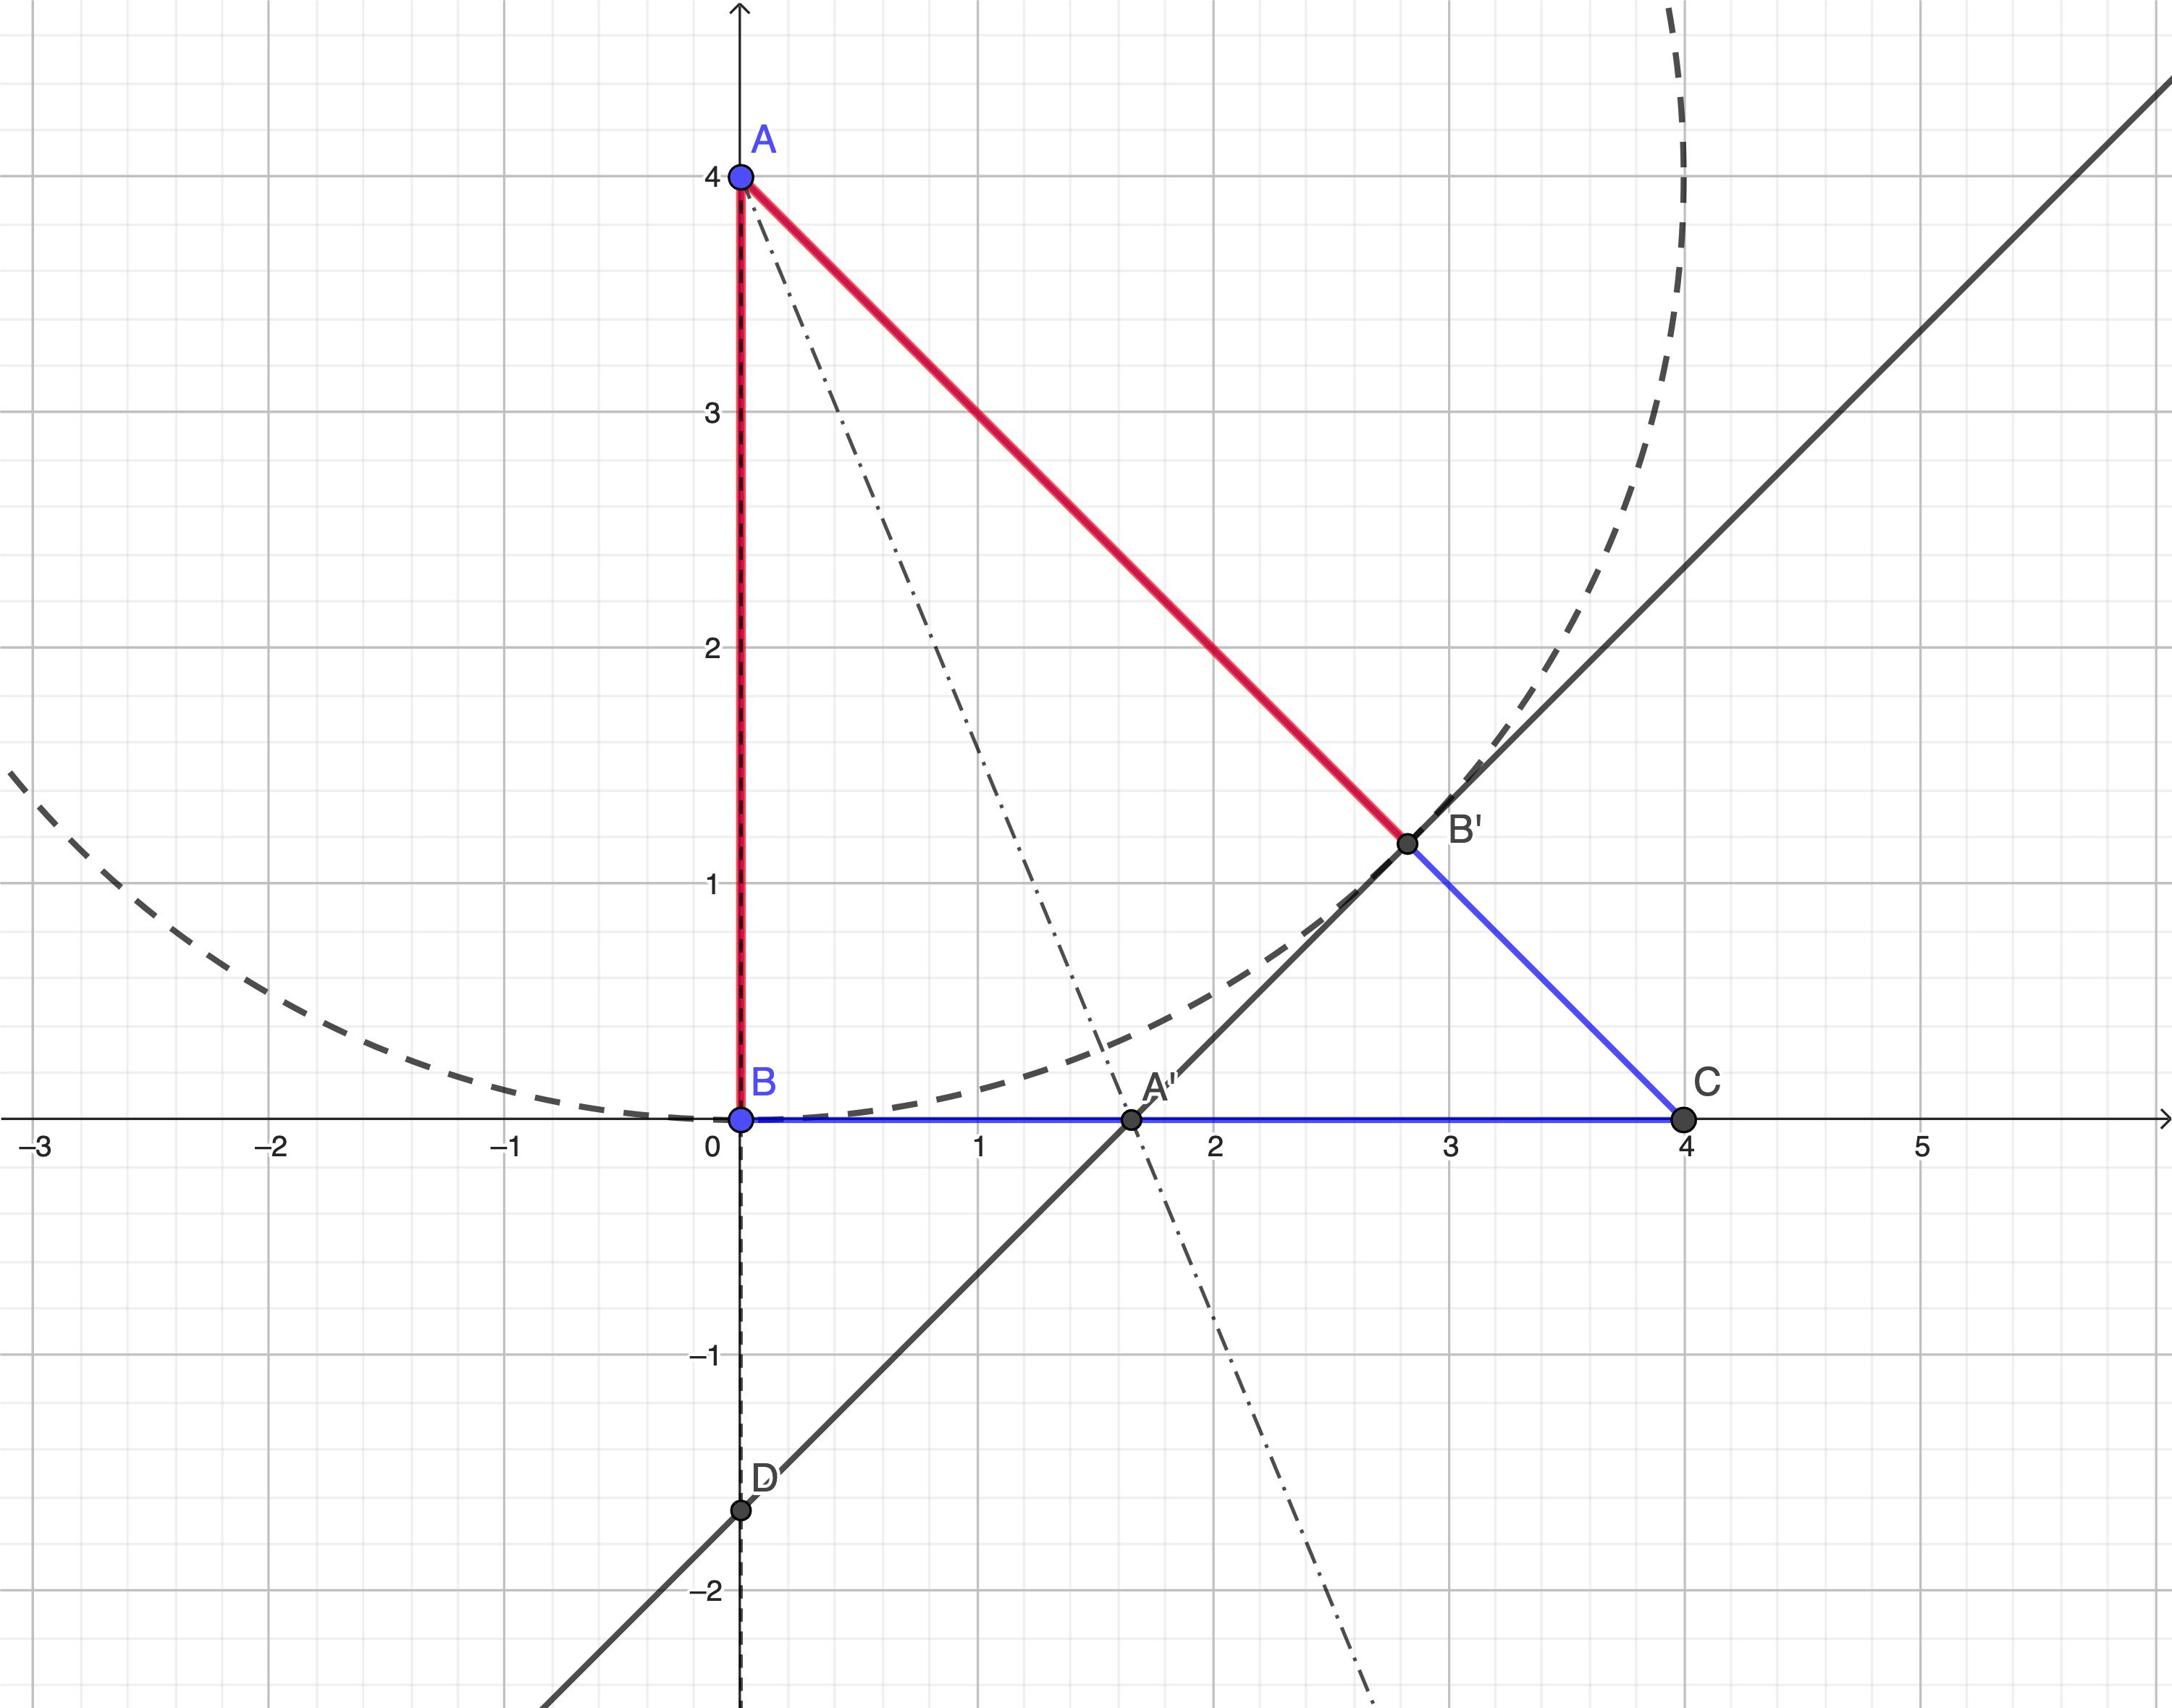
\includegraphics[width=0.85\textwidth]{./img/isorectangle-sqrt2-png.png}
\end{enumerate}



\section{Exercice}
\label{sec:orgf8bcce0}
Considérons un cube d'arête 1.
\begin{enumerate}
\item Montrer que la diagonale principale (reliant deux sommets
opposés en traversant le cube) vaut exactement \(\sqrt{3}\).
\item Montrer que \(\sqrt{3}\) est irrationnel.
\end{enumerate}


Voir solutions \ref{sec:org1db2d7e}

\section{Généralisation}
\label{sec:org8110f95}

Montrons par l'absurde que si \(p\) est un nombre premier alors
\(\sqrt{p}\) est irrationnel. \(\sqrt{p} = \frac{a}{b}\) avec \(pgcd(a,
    b) = 1\). Il vient \(a^2 = pb^2\) or \(a^2\) et \(b^2\) n'ont pas de
diviseur commun donc \(p\) divise \(a^2\) et donc \(a\). Ainsi \(a = pk\)
avec \(k\in\Z\). Par conséquent \(a^2 = p^2k^2\) et d'autre
part \(a^2 = pb^2\) d'où \(b^2 = pk^2\). Puisque \(a^2\) et \(b^2\) n'ont
pas de diviseur commun \(k^2\) ne divise pas \(b^2\). Donc c'est
forcément \(p\) d'où la contradiction.

En fait, que l'on choisisse \(k^2\) ou \(p\) comme diviseur de \(b^2\)
dans les deux cas on aboutit à une contradiction.

De plus, il y a un passage subtil ici, c'est parce que \(p\) est
premier (comme 2 et 3) que \(p\) divise \(a^2\) entraîne \(p\) divise
\(a\). Prenez le nombre 4, il divise \(2^2\) mais ne divise pas
\(2\). Ou encore 9 divise \(6^2\) mais ne divise pas 6. Donc la
primalité de \(p\) est importante sinon la démonstration est
invalide.

\section{Exercice}
\label{sec:org73038fa}
\begin{enumerate}
\item Trouver 5 contre-exemples de \(k\) divise \(a^2\) mais \(k\) ne
divise pas \(a\).
\item Montrer que \(\Phi = \frac{1 + \sqrt{5}}{2}\) est irrationnel.
\end{enumerate}


Voir solutions \ref{sec:org77e137f}

\section{Probablement irrationnel}
\label{sec:org8f6f14a}

Aussi surprenant que cela puisse paraître il y a infiniment plus
de nombres irrationnels que de rationnels. Si vous lanciez un
couteau au hasard sur une planche en bois graduée\ldots{} vous
tomberiez probablement sur un nombre irrationnel. Malheureusement
les mathématiques nécessaires pour montrer ce résultat dépasse
largement le cadre de cet ouvrage et du lycée en général. Il
faudrait invoquer des arguments d'analyse topologique à propos de
la notion de densité. Tout ça pour vous dire que l'aventure avec
les nombres réels (et les nombres en général) continue bien
au-delà des limites de ce livres. Et c'est avec regret que je suis
contraint de vous laissez sans preuve pour l'irrationalité de
\(\pi\). Voyez-vous, les arguments requis font appels aux concepts
de dérivée (que vous verrez en première), d'intégrale (que vous
verrez en terminale) et d'autres plus sophistiqués qui
interviendront dans les mathématiques du supérieur.

Espérons tout de même que la lecture de ce livre vous aura fait
découvrir la richesse des nombres réels. Si vous avez la moindre
suggestion d'amélioration merci de m'écrire à l'adresse
indiquée dans le formulaire avec pour \textbf{objet Amazon Manipuler les réels}.
\stopcontents[level-2]
\stopcontents[level-1]

\part{Capacités attendues}
\label{sec:org7810a4f}
\startcontents[level-1]
\printcontents[level-1]{}{0}{\setcounter{tocdepth}{2}}
\begin{foreigndisplayquote}{english}
To me, mathematics, computer science, and the arts are insanely
related. They’re all creative expressions.\\

\href{https://en.wikipedia.org/wiki/Sebastian\_Thrun}{Sebastian Thrun}
\end{foreigndisplayquote}

\chapter{Rappels concernant les capacités attendues}
\label{sec:org4b912db}
\startcontents[level-2]
\printcontents[level-2]{}{0}{\setcounter{tocdepth}{4}}

\begin{foreigndisplayquote}{french}
Il n’y a guère de discipline plus mal connue et plus mal décrite
que la mathématique. Combien pourraient répondre à la question :
les mathématiques ça parle de quoi ? ça porte sur quoi ? ça propose
quel but ?\\

\href{https://fr.wikipedia.org/wiki/Michel\_Demazure}{Michel Demazure}
\end{foreigndisplayquote}

Pour rappels tous les codes sont accessibles sur Google Colab à
l'adresse communiquée dans la section concernée lorsque vous
aurez rempli ce petit formulaire :
\url{https://forms.gle/pT3GVr8PdNYCeVir7} (vous trouverez également
les corrections de tous les exercices du livre).

C'est également sur Google Colab que vous pourrez tester tous les
programmes qui vous permettent de pratiquer les capacités attendues
de manière interactive.

\begin{itemize}
\item Associer à chaque point de la droite graduée un unique nombre réel
et réciproquement.
\item Représenter un intervalle de la droite numérique. Déterminer si un
nombre réel appartient à un intervalle donné.
\item Donner un encadrement, d'amplitude donnée, d'un nombre réel par
des décimaux.
\item Dans le cadre de la résolution de problèmes, arrondir en donnant
le nombre de chiffres significatifs adapté à la situation étudiée.
\end{itemize}

Tout ça se trouve sur Google Colab de façon interactive.
\stopcontents[level-2]

\chapter{\(C_1\) : Associer à chaque point de la droite graduée un unique nombre réel et réciproquement}
\label{sec:org2051646}
\startcontents[level-2]
\printcontents[level-2]{}{0}{\setcounter{tocdepth}{4}}

\begin{foreigndisplayquote}{french}
Un mathématicien est une personne capable de trouver des analogies
entre les théorèmes ; un meilleur mathématicien peut voir des
analogies entre les démonstrations. Les très bons mathématiciens
sont ceux capables de déceler des analogies entre des
théories. Mais on peut supposer que le mathématicien ultime est
celui qui peut voir des analogies entres les analogies.\\

\href{https://fr.wikipedia.org/wiki/Stefan\_Banach}{Stephan Banach}
\end{foreigndisplayquote}

\section{Code pour construire les points}
\label{sec:org7d3dc01}

Pour rappels tous les codes sont accessibles sur Google Colab à
l'adresse communiquée dans la section concernée lorsque vous
aurez rempli ce petit formulaire :
\url{https://forms.gle/pT3GVr8PdNYCeVir7} (vous trouverez également
les corrections de tous les exercices du livre).

C'est également sur Google Colab que vous pourrez tester tous les
programmes qui vous permettent de pratiquer les capacités attendues
de manière interactive.

Voici le code pour construire les points :

\begin{verbatim}
import matplotlib.pyplot as plt
import numpy as np

c_1 = "Associer à chaque point de la droite graduée "
c_1 += "un unique nombre réel et réciproquement."
print(c_1)
numbers = [-2, -0.5, 0, 1, np.sqrt(2), np.pi]
labels = ['P_0', 'P_1', 'P_2', 'P_3', 'P_4', 'P_5']

plt.figure(figsize=(10, 1))

# Ploter une ligne horizontale
plt.plot([min(numbers), max(numbers)], [0, 0], 'k')

# Placer les nombres sur la ligne graduée
plt.scatter(numbers, np.zeros_like(numbers), color='red')

# Ajouter des étiquettes aux nombres
for i, label in enumerate(labels):
    plt.text(numbers[i], 0.02, label, ha='center')

# Masquer les axes
plt.axis('off')

plt.show()
\end{verbatim}

\section{Exercice}
\label{sec:orgc3f82e5}
Voici le code pour lancer l'exercice :

\begin{verbatim}
from math import pi

nombres = {2**0.5, -2, -0.5, 1, pi, 0}
points = {'P_0': 0, 'P_1': 0, 'P_2': 0, 'P_3': 0, 'P_4': 0, 'P_5': 0}
print("Voici la liste des points dont tu vas déterminer les abscisses")
print(points)

for nb in nombres:
  p = input(f"{round(nb, 4)} correspond à l'abscisse de quel point ? ")
  points[p] = round(nb, 4)
\end{verbatim}

Voir solution \ref{sec:orgefbdf8f}
\stopcontents[level-2]

\chapter{\(C_2\) : Réprésenter un intervalle de la droite numérique. Détrminer si un nombre réel appartient à un intervalle donné}
\label{sec:orge169269}
\startcontents[level-2]
\printcontents[level-2]{}{0}{\setcounter{tocdepth}{4}}

\begin{foreigndisplayquote}{french}
Le but de la rigueur mathématique est de sanctionner et de
légitimiser les conquêtes de l'intuition, et il n'y a  jamais eu
d'autre raison de la développer.\\

\href{https://fr.wikipedia.org/wiki/Jacques\_Hadamard}{Jacques Hadamard}
\end{foreigndisplayquote}

\section{Placement des abscisses sur la droite réelle}
\label{sec:orgb0d4426}

Pour rappels tous les codes sont accessibles sur Google Colab à
l'adresse communiquée dans la section concernée lorsque vous
aurez rempli ce petit formulaire :
\url{https://forms.gle/pT3GVr8PdNYCeVir7} (vous trouverez également
les corrections de tous les exercices du livre).

C'est également sur Google Colab que vous pourrez tester tous les
programmes qui vous permettent de pratiquer les capacités attendues
de manière interactive.

Voici le code :

\begin{verbatim}
import matplotlib.pyplot as plt
import numpy as np

c_2 = "Représenter un intervalle de la droite numérique.\n"
c_2 += "Déterminer si un nombre réel appartient à un intervalle donné."
print(c_2)
numbers = [1 + i/10 for i in range(11)]
labels = [str(num) for num in numbers]

plt.figure(figsize=(10, 1))

# Ploter une ligne horizontale
plt.plot([min(numbers), max(numbers)], [0, 0], 'k')

# Placer les nombres sur la ligne graduée
plt.scatter(numbers, np.zeros_like(numbers), color='red')

# Ajouter des étiquettes aux nombres
for i, label in enumerate(labels):
    plt.text(numbers[i], 0.02, label, ha='center')

# Masquer les axes
plt.axis('off')

plt.show()
\end{verbatim}

\section{Exercice}
\label{sec:org837f3c6}
Pour rappels tous les codes sont accessibles sur Google Colab à
l'adresse communiquée dans la section concernée lorsque vous
aurez rempli ce petit formulaire :
\url{https://forms.gle/pT3GVr8PdNYCeVir7} (vous trouverez également
les corrections de tous les exercices du livre).

C'est également sur Google Colab que vous pourrez tester tous les
programmes qui vous permettent de pratiquer les capacités attendues
de manière interactive.

Voici le code pour générer l'exercice :

\begin{verbatim}
num_to_square = [1 + i/10 for i in range(5)]
list_of_intervals = []
for n2s in num_to_square:
  print(f"Dans quel intervalle appartient {n2s}**2 ?")
  interval = []
  for borne in ("inf", "sup"):
    msg = f"Borne {borne}érieure au dixième = "
    interval.append(float(input(msg)))
  list_of_intervals.append(interval)

print("Voici la liste de tes réponses")
print(list_of_intervals)
print("Voici tes correspondances")
for i in range(len(num_to_square)):
  n2s, interval = num_to_square[i], list_of_intervals[i]
  msg = f"{n2s}**2 = {round(n2s**2, 2)} appartient à "
  msg += f"l'intervalle {interval}"
  print(msg)
\end{verbatim}

Voir solution \ref{sec:org814b848}
\stopcontents[level-2]

\chapter{\(C_3\) : Donner un encadrement, d’amplitude donnée, d’un nombre réel par des décimaux}
\label{sec:orga688303}
\startcontents[level-2]
\printcontents[level-2]{}{0}{\setcounter{tocdepth}{4}}

\begin{foreigndisplayquote}{french}
La physique est écrite dans cet immense livre qui continuellement
se tient ouvert devant nos yeux (je veux dire l'univers), mais elle
ne peut se comprendre si on ne s'exerce d'abord à comprendre la
langue et à connaître les caractères avec lesquels elle est
écrite. Elle est écrite en langue mathématique, et les caractères
sont les triangles, les cercles et autres figures géométriques,
sans lesquelles il est humainement impossible d'en comprendre le
moindre mot, sans lesquelles on s'égare vainement dans un
labyrinthe obscur.\\

\href{https://fr.wikipedia.org/wiki/Galil\%C3\%A9e\_(savant)}{Galilée}
\end{foreigndisplayquote}

\section{Exercice}
\label{sec:orgba6b593}
Pour rappels tous les codes sont accessibles sur Google Colab à
l'adresse communiquée dans la section concernée lorsque vous
aurez rempli ce petit formulaire :
\url{https://forms.gle/pT3GVr8PdNYCeVir7} (vous trouverez également
les corrections de tous les exercices du livre).

C'est également sur Google Colab que vous pourrez tester tous les
programmes qui vous permettent de pratiquer les capacités attendues
de manière interactive.


Voici le code pour générer l'exercice :
\begin{verbatim}
import math

some_primes = [2, 3, 5, 7, 11, 13, 17, 19, 23, 31, 37, 41]
prime_roots = [math.sqrt(sp) for sp in some_primes]
for i in range(8, len(prime_roots)):
  inf, sup = default(prime_roots[i], i), excess(prime_roots[i], i)
  print(f"Un encadrement de √{some_primes[i]} ~", end=" ")
  print(f"{round(prime_roots[i], i)} d'amplitude 10**(-{i}) est :", end=" ")
  print(f"{inf} <= √{some_primes[i]} <= {sup}")
  print(f"Dit autrement, √{some_primes[i]} ~", end=" ")
  print(f"{round(prime_roots[i], i)}", end=" ")
  print(f"appartient à l'intervalle [{inf}; {sup}]")

def exo_amplitude():
  score, method, born = 0, [default, excess], ["inf", "sup"]
  motivation = "À toi de jouer !"
  print(motivation)
  instr = "Donne un encadrement à 10**"
  for i in range(5):
    print(f"{instr}(-{some_primes[i]}) près de √{some_primes[i]}")
    for j in range(2):
      t = method[j](prime_roots[i], some_primes[i])
      r = float(input(f"Borne {born[j]}érieure à {some_primes[i]} chiffres = "))
      if r == t:
	print("Bien joué !")
	score += 0.2
      else:
	print(f"La bonne réponse était {t}")
\end{verbatim}

Voir solutions \ref{sec:org3cfb91a}

\section{Exercice}
\label{sec:org0e68f9c}
Pour rappels tous les codes sont accessibles sur Google Colab à
l'adresse communiquée dans la section concernée lorsque vous
aurez rempli ce petit formulaire :
\url{https://forms.gle/pT3GVr8PdNYCeVir7} (vous trouverez également
les corrections de tous les exercices du livre).

C'est également sur Google Colab que vous pourrez tester tous les
programmes qui vous permettent de pratiquer les capacités attendues
de manière interactive.


Voici le code pour générer l'exercice :
\begin{verbatim}
def approx_nums(some_numbers, decimals):
  score, method, born = 0, [default, excess], ["inf", "sup"]
  motivation = "À toi de jouer !"
  print(motivation)
  instr = "Donne un encadrement à 10**"
  for num in some_numbers:
    boundaries = [default(num, decimals), excess(num, decimals)]
    print(f"{instr}(-{decimals}) près de {num}")
    for j in range(2):
      t = boundaries[j]
      r = float(input(f"Borne {born[j]}érieure à {decimals} chiffres = "))
      if r == t:
	print("Bien joué !")
	score += 1
      else:
	print(f"La bonne réponse était {t}")
    x_pts, inf, sup, d = num, boundaries[0], boundaries[1], decimals
    step = 10**(-decimals)
    zoom(x_pts, inf, sup, step, decimals, size=(9.75, 1.25))
  print(f"Score final = {score * 10}%")


phi = (1 + 5**0.5) / 2 # nombre d'or
print(f"On appelle nombre d'or et on le note ɸ = (1 + √5) / 2 ~ {phi}")
phi2, tau = phi**2, 2 * math.pi
print("Vous pouvez remarquer que ɸ**2 = 1 + ɸ (vérifiez-le par le calcul !)")
print(f"On appelle 𝛕 = 2π ~ {tau}")
print(f"On ne présente plus π ~ {math.pi}")
print(f"On appelle constante d'Euler e ~ {math.e}")
some_numbers = [phi, phi2, math.e, math.pi, tau]
decimals = random.randint(2, 5)
approx_nums(some_numbers, decimals)
\end{verbatim}

Voir solutions \ref{sec:org7cc2be4}
\stopcontents[level-2]

\chapter{\(C_4\) : Dans le cadre de la résolution de problèmes, arrondir en donnant le nombre de chiffres significatifs adapté à la situation étudiée}
\label{sec:orge07749d}
\startcontents[level-2]
\printcontents[level-2]{}{0}{\setcounter{tocdepth}{4}}

\begin{foreigndisplayquote}{french}
Tout mathématicien digne de ce nom a connu, parfois seulement à de
rares intervalles, ces états d’exaltation lucide où les pensées
s’enchaînent comme par miracle, et où l’inconscient (quel que soit
le sens qu’on attache à ce mot) paraît aussi avoir sa part. [\ldots{}] A
la différence du plaisir sexuel, celui-là peut durer plusieurs
heures, voire plusieurs jours ; qui l’a connu en désire le
renouvellement mais est impuissant à le provoquer, sinon tout au
plus par un travail opiniâtre dont il apparaît alors comme la
récompense ; il est vrai que le plaisir qu’on en ressent est sans
rapport avec la valeur des découvertes auxquelles il s’associe.\\

\href{https://fr.wikipedia.org/wiki/Andr\%C3\%A9\_Weil}{André Weil}
\end{foreigndisplayquote}

\section{Exemple}
\label{sec:orga5b1cb5}
Pour rappels tous les codes sont accessibles sur Google Colab à
l'adresse communiquée dans la section concernée lorsque vous
aurez rempli ce petit formulaire :
\url{https://forms.gle/pT3GVr8PdNYCeVir7} (vous trouverez également
les corrections de tous les exercices du livre).

C'est également sur Google Colab que vous pourrez tester tous les
programmes qui vous permettent de pratiquer les capacités attendues
de manière interactive.

Voici le code pour générer l'exemple :
\begin{verbatim}
c = 299_792_458
print(f"La vitesse de la lumière dans le vide est de {c} mètres par seconde.")
e_s = "L'écriture scientifique d'un nombre n = a x 10**k"
e_s += "\na appartient à l'intervalle [1; 10[ donc a < 10"
e_s += "\nk appartient à l'ensemble des entiers relatifs"
a, k = 2.99792458, 8
print(f"Son écriture scientifique est c = {a} x 10**{k} m/s")
print("Pour passer des mètres aux kilomètres il faut diviser par 1 000")
print("Cela revient à multiplier par 10**(-3)")
print(f"D'où c = {a} x 10**{k-3} km/s")
print("Dans 1 heure il y 60 minutes et dans 1 minute il y a 60 secondes")
print("Donc dans 1 heure il y 60 x 60 = 3600 secondes")
print("Donc il faut multiplier par 3600")
print("Mais dans ce cas, autant faire d'une pierre, deux coups")
print("Multiplier par 3600 et diviser par 1 000 revient à multiplier par 3.6")
a *= 3.6
if a > 10:
  a /= 10
  k -= 1
print(f"D'où c = {a} x 10**{k} km/h")
\end{verbatim}

\section{Exercice}
\label{sec:org329206f}
Pour rappels tous les codes sont accessibles sur Google Colab à
l'adresse communiquée dans la section concernée lorsque vous
aurez rempli ce petit formulaire :
\url{https://forms.gle/pT3GVr8PdNYCeVir7} (vous trouverez également
les corrections de tous les exercices du livre).

C'est également sur Google Colab que vous pourrez tester tous les
programmes qui vous permettent de pratiquer les capacités attendues
de manière interactive.

Voici le code pour générer l'exercice :
\begin{verbatim}
print("À toi de jouer !")
mile = 1609.344
print(f"Sachant que 1 mile = {mile} mètres")
print("Calcule la vitesse de la lumière en miles par heure.")
msg = "Prend le temps de poser les calculs sur un papier avant de répondre"
print(msg.upper())
user_rep = float(input("Vitesse en miles par heure = "))
print(f"Selon toi c = {user_rep} mph (miles per hour)")
\end{verbatim}
\stopcontents[level-2]
\stopcontents[level-1]

\part{Démonstrations}
\label{sec:org2c84789}
\startcontents[level-1]
\printcontents[level-1]{}{0}{\setcounter{tocdepth}{2}}
\begin{foreigndisplayquote}{english}
The pure mathematician, like the musician, is a free creator of his
world of ordered beauty.\\

\href{https://amzn.to/3ONEWLI}{Bertrand Russell}
\end{foreigndisplayquote}

\chapter{Rappels des éléments du programme officiel}
\label{sec:orgaf7bf45}
\startcontents[level-2]
\printcontents[level-2]{}{0}{\setcounter{tocdepth}{4}}

\begin{foreigndisplayquote}{french}
Une théorie mathématique ne peut être considérée comme complète
tant que l'on ne l'a clarifiée au point de pouvoir l'expliquer au
premier homme que l'on croise dans la rue.\\

\href{https://fr.wikipedia.org/wiki/David\_Hilbert}{David Hilbert}  
\end{foreigndisplayquote}

Les deux démonstrations au programme concernent :
\begin{itemize}
\item Le nombre rationnel \(\frac{1}{3}\) n'est pas décimal.
\item Le nombre réel \(\sqrt{2}\) est irrationnel.
\end{itemize}

Ces deux démonstrations sont traitées sur Google Colab.

Pour rappels tous les codes sont accessibles sur Google Colab à
l'adresse communiquée dans la section concernée lorsque vous
aurez rempli ce petit formulaire :
\url{https://forms.gle/pT3GVr8PdNYCeVir7} (vous trouverez également
les corrections de tous les exercices du livre).
\stopcontents[level-2]

\chapter{Démonstrations pour \(\frac{1}{3}\)}
\label{sec:org9a945ab}
\startcontents[level-2]
\printcontents[level-2]{}{0}{\setcounter{tocdepth}{4}}

\begin{foreigndisplayquote}{french}
Quel que soit le temps passé à faire des mathématiques, ce n'est
jamais du temps perdu.\\

\href{https://fr.wikipedia.org/wiki/C\%C3\%A9dric\_Villani}{Cédric Villani}
\end{foreigndisplayquote}

\section{À la main}
\label{sec:orgcc94390}

Mais proposons une démonstration utilisant l'astuce des nombres à
décimales périodiques vue dans \ref{sec:org67927a1}.

Posons \(x = 0,3\dots 3\) où 3 se répète à l'infini. Multiplions par
10 puis retranchons \(x\). Ainsi \(9x = 3\) donc \(x = \frac{1}{3}\). CQFD

Pour \(\sqrt{2}\) consulter Google Colab ou les démonstrations
précédentes.

En espérant que la lecture de ce livre vous aura satisfait et fait
découvrir la richesse des nombres réels. Si vous avez la moindre
suggestion d'amélioration merci de m'écrire à l'adresse
indiquée dans le formulaire avec pour \textbf{objet Amazon Manipuler les réels}.

\section{Avec Python}
\label{sec:orge021a52}

Pour rappels tous les codes sont accessibles sur Google Colab à
l'adresse communiquée dans la section concernée lorsque vous
aurez rempli ce petit formulaire :
\url{https://forms.gle/pT3GVr8PdNYCeVir7} (vous trouverez également
les corrections de tous les exercices du livre).

Voici le code pour générer les 3 démonstrations :
\begin{verbatim}
def read_text(txt):
  for t in txt:
    input(f"{t}\nAppuyez sur une touche pour lire la suite...")


intro = [
    "Le nombre 1/3 est-il décimal ?",
    "Pour que 1/3 soit décimal",
    "il faudrait trouver a et n tels que 1/3 = a/10**n.",
    "En faisant un produit en croix cela revient à 10**n = 3*a.",
    "Maintenant le problème devient beaucoup plus simple.",
    "Il suffit de prouver qu'aucune puissance de 10 n'est mulitple de 3."
    ]

read_text(txt=intro)

multiple_of_3 = [3*k for k in range(21)]
print("Voici les multiples de 0 à 60")
print(multiple_of_3)
rem = input("Que remarquez-vous ? ")
more = input("Vous en voulez plus ? 0) Non 1) Oui\n")
if more == "1":
  for k in range(21, 50):
    print(3*k, end=", ")
  print()

div = input("Quels sont les diviseurs (entiers positifs) de 10 ? ")
div = div.split(",")
div = [int(d) for d in div]
print(f"Selon vous, les diviseurs de 10 sont {div}")
prime_proof = [
    "Les diviseurs de 10 sont 2 et 5",
    "Donc les diviseurs de n'importe quelle puissance de 10",
    "sont de la forme 2**p x 5**q",
    "avec p et q tels que p + q <= n",
    "Aucune puissance de 2 ne divise 3",
    "car 2 et 3 sont premiers entre eux (ils n'ont pas de diviseurs communs)",
    "il en va de même pour 5 et 3",
    "donc il est impossible d'obtenir 10**n = 3*a",
    "une autre façon de faire consiste à poser la division de 10 par 3",
    "vous constaterez qu'il y aura toujours un reste non nul",
    "et vous pourriez faire de même à l'infini avec toute puissance de 10"
]

read_text(txt=prime_proof)

div_proof = [f"10**{n} = 3 x {(10**n)//3} + {(10**n) % 3}" for n in range(10)]
read_text(txt=div_proof)

decimal_proof = [f"1/3 ~ {round(1/3, i)} à {i} décimale(s)" for i in range(10)]
read_text(txt=decimal_proof)

magic_proof = [
    "Supposons qu'il existe un nombre noté x = 0.333333...",
    "Puisqu'il y a une infinité de 3 après la virgule alors",
    "10x = 3.333333... avec une infinité de 3 après la virgule",
    "10x - x = 3 et donc 9x = 3 d'où x = 3/9 = 1/3",
    "CQFD"
]
read_text(txt=magic_proof)
\end{verbatim}
\stopcontents[level-2]
\stopcontents[level-1]

\part{Exemple d'algorithme}
\label{sec:org283c364}
\startcontents[level-1]
\printcontents[level-1]{}{0}{\setcounter{tocdepth}{2}}
\begin{foreigndisplayquote}{english}
Just because we can’t find a solution, it doesn’t mean there isn’t
one.\\

\href{https://en.wikipedia.org/wiki/Andrew\_Wiles}{Andrew Wiles}
\end{foreigndisplayquote}

\chapter{Rappel des éléments du programme officiel}
\label{sec:org2cc4231}
\startcontents[level-2]
\printcontents[level-2]{}{0}{\setcounter{tocdepth}{4}}

\begin{foreigndisplayquote}{french}
Monsieur Fourier avait l'opinion que le but principal des
mathématiques était l'utilité publique et l'explication des
phénomènes naturels. Un philosophe tel que lui aurait dû savoir que
le but unique de la Science, c'est l'honneur de l'esprit humain et
que, sous ce titre, une question de nombres vaut bien une question
de système du monde.\\

\href{https://fr.wikipedia.org/wiki/Charles\_Gustave\_Jacob\_Jacobi}{Charles Gustave Jacob Jacobi}
\end{foreigndisplayquote}

Le programme officiel propose un seul exemple d'algorithme :
\begin{itemize}
\item Déterminer par balayage un encadrement de \(\sqrt{2}\) d'amplitude
inférieure ou égale à \(10^{-n}\).
\end{itemize}
\stopcontents[level-2]

\chapter{Petites explications}
\label{sec:org3c07af2}
\startcontents[level-2]
\printcontents[level-2]{}{0}{\setcounter{tocdepth}{4}}

\begin{foreigndisplayquote}{french}
Les mathématiques ont des inventions très subtiles et qui peuvent
beaucoup servir, tant à contenter les curieux qu'à faciliter tous
les arts et à diminuer le travail des hommes. \\

\href{https://fr.wikipedia.org/wiki/Ren\%C3\%A9\_Descartes}{René Descartes}
\end{foreigndisplayquote}

On cherche des réels \(a\) et \(b\) tels que \(a < \sqrt{2} < b\) avec
\(\lvert a - b \rvert \leq 10^{-n}\).

Comme \(\sqrt{2} \geq 1\) alors on va choisir \(a \geq 1\).

De sorte que \(a^2 \leq 2 \leq b^2\).
\stopcontents[level-2]

\chapter{Le code}
\label{sec:org5c6ef71}
\startcontents[level-2]
\printcontents[level-2]{}{0}{\setcounter{tocdepth}{4}}

\begin{foreigndisplayquote}{french}
Si vous touchez aux maths, vous ne devez être ni pressés, ni
cupides, fussiez-vous roi ou reine. \\

\href{https://amzn.to/3KU1CZE}{Euclide} 
\end{foreigndisplayquote}

Voici le code que vous pouvez retrouver sur Google Colab :

\begin{verbatim}
def balayage(n):
  """
  Cette fonction renvoie les bornes d'un encadrement par balayage
  d'amplitude inférieure ou égale à 10**(-n)
  """
  a = 1
  b = a + 10**(-n)
  while b**2 < 2:
    a += 10**(-n)
    b = a + 10**(-n)
  return round(a, n), round(b, n)

# Tests : attention parce qu'au-delà de n = 7 ça devient très long 
for n in range(1, 7):
  infimum, supremum = balayage(n)
  ampli = 10**(-n)
  print(f"{infimum} < √2 < {supremum} est un encadrement d'amplitude {ampli}")
\end{verbatim}

Pour rappels tous les codes sont accessibles sur Google Colab à
l'adresse communiquée dans la section concernée lorsque vous
aurez rempli ce petit formulaire :
\url{https://forms.gle/pT3GVr8PdNYCeVir7} (vous trouverez également
les corrections de tous les exercices du livre).

En espérant que la lecture de ce livre vous aura satisfait et fait
découvrir la richesse des nombres réels. Si vous avez la moindre
suggestion d'amélioration merci de m'écrire à l'adresse
indiquée dans le formulaire avec pour \textbf{objet Amazon Manipuler les réels}.
\stopcontents[level-2]
\stopcontents[level-1]

\part{Approfondissements possibles}
\label{sec:org37588f5}
\startcontents[level-1]
\printcontents[level-1]{}{0}{\setcounter{tocdepth}{2}}
\begin{foreigndisplayquote}{english}
Millions saw the apple fall, but Newton asked why.\\

\href{https://en.wikipedia.org/wiki/Bernard\_Baruch}{Bernard Baruch}
\end{foreigndisplayquote}

\chapter{Rappel des éléments du programme officiel}
\label{sec:org31d8817}
\startcontents[level-2]
\printcontents[level-2]{}{0}{\setcounter{tocdepth}{4}}

\begin{foreigndisplayquote}{french}
Les mathématiques sont une gymnastique de l'esprit et une
préparation à la philosophie. \\

\href{https://fr.wikipedia.org/wiki/Isocrate}{Isocrate}
\end{foreigndisplayquote}

D'apprès le programme officiel les approfondissements possibles
sont :
\begin{itemize}
\item Développement décimal illimité d'un nombre réel.
\item Observation, sur des exemples, de la périodicité du développement
décimal de nombres rationnels, du gait qu'un développement décimal
périodique correspond à un rationnel.
\end{itemize}
\stopcontents[level-2]

\chapter{Petit bilan}
\label{sec:org2b46cf0}
\startcontents[level-2]
\printcontents[level-2]{}{0}{\setcounter{tocdepth}{4}}

\begin{foreigndisplayquote}{french}
Il y a une joie réelle à faire des mathématiques, à apprendre de
nouvelles méthodes de pensée qui expliquent, organisent et
simplifient. On peut ressentir cette joie en découvrant de
nouvelles mathématiques, (…) ou en trouvant une nouvelle façon
d’expliquer (…) une structure mathématique ancienne. \\

\href{https://en.wikipedia.org/wiki/William\_Thurston}{William P. Thurston}
\end{foreigndisplayquote}

Pour le deuxième point on a déjà vu beaucoup d'exemple (cf la petite
astuce vue dans \ref{sec:org67927a1}).

Mais rien que pour le plaisir en voici encore un. Soit \(x =
  0,2023\dots\). Ici la période est 2023. Donc on va multiplier par
\(10^4\) puis retrancher \(x\) d'où \(9999x = 2023\) qui entraîne \(x =
  \frac{2023}{9999} \simeq 0,2023\dots 2023\dots\)
\stopcontents[level-2]

\chapter{Et pour quelques exemples de plus}
\label{sec:orgdfc5b8e}
\startcontents[level-2]
\printcontents[level-2]{}{0}{\setcounter{tocdepth}{4}}

\begin{foreigndisplayquote}{english}
Pure mathematics is, in its way, the poetry of logical ideas.\\
\href{https://en.wikipedia.org/wiki/Albert\_Einstein}{Albert Einstein}   
\end{foreigndisplayquote}

Voici quelques développement décimaux illimités de nombres réels :

\begin{align*}
\sqrt{2} &\simeq 1,414213562373095\dots\\
\Phi &\simeq 1.618033988749895\dots\\
\sqrt{3} &\simeq 1.7320508075688772\dots\\
\sqrt{5} &\simeq 2.23606797749979\dots\\
\sqrt{7} &\simeq 2.6457513110645907\dots\\
e &\simeq 2.718281828459045\dots\\
\pi &\simeq 3.141592653589793\dots \\
\sqrt{11} &\simeq 3.3166247903554\dots
\end{align*}

En espérant que la lecture de ce livre vous aura satisfait et fait
découvrir la richesse des nombres réels. Si vous avez la moindre
suggestion d'amélioration merci de m'écrire à l'adresse
indiquée dans le formulaire avec pour \textbf{objet Amazon Manipuler les réels}.
\stopcontents[level-2]
\stopcontents[level-1]

\part{Après ce livre}
\label{sec:org877c75b}
\startcontents[level-1]
\printcontents[level-1]{}{0}{\setcounter{tocdepth}{2}}
\begin{foreigndisplayquote}{english}
I’ve always been interested in using mathematics to make the world
work better.\\

\href{https://en.wikipedia.org/wiki/Alvin\_E.\_Roth}{Alvin E. Roth}
\end{foreigndisplayquote}

\chapter{Conclusion}
\label{sec:org2d74712}
\startcontents[level-2]
\printcontents[level-2]{}{0}{\setcounter{tocdepth}{4}}

\begin{foreigndisplayquote}{english}
Without mathematics, there’s nothing you can do. Everything around
you is mathematics. Everything around you is numbers.\\

\href{https://en.wikipedia.org/wiki/Shakuntala\_Devi}{Shakuntala Devi} 
\end{foreigndisplayquote}

Bravo à vous si vous avez lu jusqu'au bout.

Pour rappels tous les codes sont accessibles sur Google Colab à
l'adresse communiquée dans la section concernée lorsque vous
aurez rempli ce petit formulaire :
\url{https://forms.gle/pT3GVr8PdNYCeVir7} (vous trouverez également
les corrections de tous les exercices du livre).

Sur Google Colab vous pourrez expérimentez avec des exercices
nouveaux à chaque exécution du code. Cela vous permettra de vous
entraîner avec des valeurs différentes à chaque fois. C'est beaucoup
plus interactifs que tous les exemples de ce livre.

Le but de ce livre est de vous donner un aperçu du monde merveilleux
des nombres réels. Mais il y a encore beaucoup de choses à découvrir
que je n'ai même pas pu mentionner ici.

Je vous invite à mettre le maximum d'étoiles sur Amazon et à laisser
un commentaire pour aider les gens qui cherchent des ressources utiles.

En espérant que la lecture de ce livre vous aura satisfait et fait
découvrir la richesse des nombres réels. Si vous avez la moindre
suggestion d'amélioration merci de m'écrire à l'adresse
indiquée dans le formulaire avec pour \textbf{objet Amazon Manipuler les réels}.
\stopcontents[level-2]
\stopcontents[level-1]

\part{Solutions des exercices de la section : \ref{sec:org4370264}}
\label{sec:orga610f4f}
\startcontents[level-1]
\printcontents[level-1]{}{0}{\setcounter{tocdepth}{2}}
\begin{foreigndisplayquote}{english}
The only way to learn mathematics is to do mathematics.\\

\href{https://en.wikipedia.org/wiki/Paul\_Halmos}{Paul Richard Halmos}
\end{foreigndisplayquote}

\chapter{Solutions des exercices de la section : \ref{sec:org4798595}}
\label{sec:org4bb3cd3}
\startcontents[level-2]
\printcontents[level-2]{}{0}{\setcounter{tocdepth}{4}}

\begin{foreigndisplayquote}{english}
We will always have STEM with us. Some things will drop out of the
public eye and go away, but there will always be science,
engineering, and technology. And there will always, always be
mathematics.\\

\href{https://en.wikipedia.org/wiki/Katherine\_Johnson}{Creola Katherine Coleman}
\end{foreigndisplayquote}

\section{Solution de l'exercice \ref{sec:org02c154b}}
\label{sec:org9049a7b}
On reprend le même schéma que dans \ref{sec:org298f45f}

\begin{align*}
A &=\,"x < -1"\\
B &=\,"-3x > 3"\\
P &=\,A\Rightarrow B\\
\neg B &=\, "-3x \leq 3"\\
\neg A &=\, "x \geq -1"\\
CP(P) &=\,(\neg B)\Rightarrow(\neg A)
\end{align*}

\section{Solution Python de l'exercice \ref{sec:orga38a814}}
\label{sec:org49e8be4}
Voir énoncé \ref{sec:orga38a814}

\begin{enumerate}
\item Pour rappels tous les codes sont accessibles sur Google Colab à
l'adresse communiquée dans la section concernée lorsque vous
aurez rempli ce petit formulaire :
\url{https://forms.gle/pT3GVr8PdNYCeVir7} (vous trouverez également
les corrections de tous les exercices du livre).

Voici le code de la fonction \texttt{imply}

\begin{verbatim}
def imply(A, B):
  """
  Cette fonction prend 2 paramètres A et B en entrée 
  et renvoie la phrase logique A implique B
  """
  return f"({A}) implique ({B})"

# Tests
A = ["x > 2", "x < -1"]
B = ["2*x > 4", "-3*x > 3"] 
for i in range(len(A)):
  print(imply(A[i], B[i]))

# Sorties
#(x > 2) implique (2*x > 4)
#(x < -1) implique (-3*x > 3)
\end{verbatim}
\item 1. Pour rappels tous les codes sont accessibles sur Google Colab à
l'adresse communiquée dans la section concernée lorsque vous
aurez rempli ce petit formulaire :
\url{https://forms.gle/pT3GVr8PdNYCeVir7} (vous trouverez également
les corrections de tous les exercices du livre).

Voici le code de la fonction \texttt{contrapose}

\begin{verbatim}
def contrapose(A, B):
  """
  Cette fonction prend 2 paramètres A et B en entrée 
  et renvoie la phrase logique non B implique non A
  """
  return imply("non " + B, "non " + A)

# Tests
A = ["x > 2", "x < -1"]
B = ["2*x > 4", "-3*x > 3"] 
for i in range(len(A)):
  print(contrapose(A[i], B[i]))

# Sorties
#(non 2*x > 4) implique (non x > 2)
#(non -3*x > 3) implique (non x < -1)
\end{verbatim}
\end{enumerate}
\stopcontents[level-2]

\chapter{Solutions des exercices de la section : \ref{sec:org7096b61}}
\label{sec:org9336dcc}
\startcontents[level-2]
\printcontents[level-2]{}{0}{\setcounter{tocdepth}{4}}

\begin{foreigndisplayquote}{english}
Mathematics as an expression of the human mind reflects the active
will, the contemplative reason, and the desire for aesthetic
perfection. Its basic elements are logic and intuition, analysis
and construction, generality and individuality.\\

\href{https://en.wikipedia.org/wiki/Richard\_Courant}{Richard Courant}
\end{foreigndisplayquote}

\section{Solutions de l'exercice \ref{sec:org3ebd799}}
\label{sec:org0af5bba}
Voir énoncé \ref{sec:org3ebd799}

\begin{enumerate}
\item \[\dfrac{1}{3}\in I_1 = [0,3 ; 0,4]\] qui a pour amplitude \[|I_1|
      = 0,4 - 0,3 = 0,1 = 10^{-1}\]
\[\dfrac{1}{3}\in I_2 = [0,33 ; 0,34]\] qui a pour amplitude
\[|I_2| = 0,34 - 0,33 = 0,01 = 10^{-2}\]
\[\dfrac{1}{3}\in I_3 = [0,333 ; 0,334]\] qui a pour amplitude
\[|I_3| = 0,334 - 0,333 = 0,001 = 10^{-3}\]
On peut classer ces intervalles :\[\dfrac{1}{3}\in I_3 = [0,333 ;
      0,334] \subset I_2 = [0,33 ; 0,34] \subset I_1 = [0,3 ; 0,4]\]
\item \[\sqrt{2}\in R_1 = [1,4 ; 1,5]\] qui a pour amplitude \[|R_1| =
      1,5 - 1,4 = 0,1 = 10^{-1}\]
\[\sqrt{2}\in R_2 = [1,41 ; 1,42]\] qui a pour amplitude \[|R_2| =
      1,42 - 1,41 = 0,01 = 10^{-2}\]
\[\sqrt{2}\in R_3 = [1,414 ; 1,415]\] qui a pour amplitude \[|R_3|
      = 1,415 - 1,414 = 0,001 = 10^{-3}\]
On peut classer ces intervalles :\[\sqrt{2}\in R_3 = [1,414 ;
      1,415] \subset R_2 = [1,41 ; 1,42]\subset R_1 = [1,4 ; 1,5]\]
\item \[\Phi = \dfrac{1 + \sqrt{5}}{2}\in F_1 = [1,6 ; 1,7]\] qui pour
amplitude \[|F_1| = 1,7 - 1,6 = 0,1 = 10^{-1}\]
\[\Phi = \dfrac{1 + \sqrt{5}}{2}\in F_2 = [1,61 ; 1,62]\] qui pour
amplitude \[|F_2| = 1,62 - 1,61 = 0,01 = 10^{-2}\]
\[\Phi = \dfrac{1 + \sqrt{5}}{2}\in F_3 = [1,618 ; 1,619]\] qui pour
amplitude \[|F_3| = 1,619 - 1,618 = 0,001 = 10^{-3}\]
On peut classer ces intervalles :\[\Phi = \dfrac{1 +
      \sqrt{5}}{2}\in F_3 = [1,618 ; 1,619] \subset F_2 = [1,61 ;
      1,62]\subset F_1 = [1,6 ; 1,7]\]
\item \[\pi\in P_1 = [3,1 ; 3,2]\] qui a pour amplitude \[|P_1| = 3,2 -
      3,1 = 0,1 = 10^{-1}\]
\[\pi\in P_2 = [3,14 ; 3,15]\] qui a pour amplitude \[|P_2| = 3,15 -
      3,14 = 0,01 = 10^{-2}\]
\[\pi\in P_3 = [3,141 ; 3,142]\] qui a pour amplitude \[|P_3| = 3,142 -
      3,141 = 0,001 = 10^{-3}\]
On peut classer ces intervalles : \[\pi\in P_3 = [3,141 ;
      3,142]\subset P_2 = [3,14 ; 3,15]\subset P_1 = [3,1 ; 3,2]\]
\item \[\tau = 2\pi\in T_1 = [6,2 ; 6,3]\] qui a pour amplitude \[|T_1| = 6,3 -
      6,2 = 0,1 = 10^{-1}\]
\[\tau = 2\pi\in T_2 = [6,28 ; 6,29]\] qui a pour amplitude \[|T_2| = 6,29 -
      6,28 = 0,01 = 10^{-2}\]
\[\tau = 2\pi\in T_3 = [6,283 ; 6,284]\] qui a pour amplitude \[|T_3| = 6,284 -
      6,283 = 0,001 = 10^{-3}\]
On peut classer ces intervalles : \[\tau = 2\pi\in T_3 = [6,283 ;
      6,284]\subset T_2 = [6,28 ; 6,29]\subset T_1 = [6,2 ; 6,3]\]
\end{enumerate}

\section{Solutions de l'exercice \ref{sec:orgddaeb73}}
\label{sec:org5140565}
Voir énoncé \ref{sec:orgddaeb73}

\begin{enumerate}
\item \[\Phi = \dfrac{1 + \sqrt{5}}{2} \simeq 1,61803\]
\item Voici les 16 premiers termes de cette suite de nombres :

\begin{align*}
F_1 = 1&& F_2 = 1&& F_3 = 2&& F_4 = 3\\
F_5 = 5&& F_6 = 8&& F_7 = 13&& F_8 = 21\\
F_9 = 34&& F_{10} = 55&& F_{11} = 89&& F_{12} = 144\\
F_{13} = 233&& F_{14} = 377&& F_{15} = 610&& F_{16} = 987
\end{align*}

\item Pour calculer un nouveau terme on ajoute les deux termes
précédents \[F_n = F_{n - 1} + F_{n-2}\]
Par exemple \(F_3 = F_2 + F_1 = 1 + 1 = 2\) ou encore \(F_7 =
       F_6 + F_5 = 8 + 5 = 13\).
\item \begin{align*}
\frac{F_2}{F_1} = 1&& \frac{F_3}{F_2} = 2\\
\frac{F_4}{F_3} = \frac{3}{2}&& \frac{F_5}{F_4} =
\frac{5}{3}\simeq 1,67\\
\frac{F_6}{F_5} = \frac{6}{5} = 1,2&&\frac{F_7}{F_6} =
\frac{13}{8} = 1,625\\
\frac{F_8}{F_7} = \frac{21}{13}\simeq
1,615&&\frac{F_9}{F_8}\simeq 1,619\\
\dfrac{F_{10}}{F_9} = \frac{55}{34}\simeq 1,6176&&
\frac{F_{11}}{F_{10}} = \frac{89}{55} = 1,6182
\end{align*}
\item Les 11 premiers termes de la suites de Fibonacci ont permis
d'approcher le nombre d'or à 3 chiffres après la
virugle. Poursuivons avec ce que nous avons déjà calculer à la
question 2.
\begin{align*}
\frac{F_{12}}{F_{11}} = \frac{144}{89}\simeq 1,6180&&\frac{F_{13}}{F_{12}} = \frac{233}{144}\simeq 1,61801\\
\frac{F_{14}}{F_{13}} = \frac{377}{233}\simeq 1,61803&&\frac{F_{15}}{F_{14}} = \frac{610}{377}\simeq 1,61804
\end{align*}
\[\Phi = \dfrac{1 + \sqrt{5}}{2} \simeq 1,61803\in
       \left[\dfrac{F_{14}}{F_{13}} ; \dfrac{F_{15}}{F_{14}}\right]\]
\end{enumerate}

\section{Solution du petit jeu \ref{sec:orgb808075}}
\label{sec:org4a65d03}
Voir énoncé \ref{sec:orgb808075}

\begin{enumerate}
\item Partie 1
\label{sec:org6955e76}

Voilà pour la première partie de la question

\begin{enumerate}
\item \[u = 0,1\dots\in I_u = [0,09 ; 0,19]\] en effet \[|I_u| = 0,19 - 0,09 = 0,1\]
\item \[v = 0,12\dots\in I_v = [0,118 ; 0,128]\] en effet \[|I_v| = 0,128 - 0,118 =
      0,01\]
\item \[w = 0,123\dots\in I_w = [0,1227 ; 0,1237]\] en effet \[|I_w| = 0,1237 - 0,1227
      = 0,001\]
\item \[x = 0,1234\dots\in I_x = [0,12336 ; 0,12346]\] en effet \[|I_x| =
      0,12346 - 0,12336 = 0,0001\]
\item \[y = 0,12345\dots\in I_y = [0,123455 ; 0,123465]\] en effet
\[|I_y| = 0,123465 - 0,123455 = 0,0001\]
\end{enumerate}

\item Partie 2
\label{sec:org8c12fbe}

Maintenant occupons-nous de la seconde partie.

\begin{enumerate}
\item \[10u = 1,1\dots\] donc \[10u - u = 1\] d'où \[u = \dfrac{1}{9}\in
      I_u = [0,09 ; 0,19]\]
\item \[100v = 12,12\dots\] donc \[100v - v = 12\] d'où \[v = \dfrac{12}{99}
      = \dfrac{4}{33}\in I_v = [0,118 ; 0,128]\]
\item \[1000w = 123,123\dots\] donc \[1000w - w = 123\] d'où \[w =
      \dfrac{123}{999} = \dfrac{41}{333}\in I_w = [0,1227 ; 0,1237]\]
\item \[10000x = 1234,1234\dots\] donc \[10000x - x = 1234\] d'où \[x =
      \dfrac{1234}{9999}\in I_x = [0,12336 ; 0,12346]\]
\item \[100000y = 12345,12345\dots\] donc \[100000y - y = 12345\] d'où \[y
      = \dfrac{12345}{99999}\in I_y = [0,123455 ; 0,123465]\]
\end{enumerate}
\end{enumerate}
\stopcontents[level-2]

\chapter{Solutions des exercices de la section : \ref{sec:org709c246}}
\label{sec:orgfa5829f}
\startcontents[level-2]
\printcontents[level-2]{}{0}{\setcounter{tocdepth}{4}}

\begin{foreigndisplayquote}{english}
Mathematics is the music of reason.\\

\href{https://en.wikipedia.org/wiki/James\_Joseph\_Sylvester}{James Joseph Sylvester}
\end{foreigndisplayquote}

\section{Solution de l'exercice \ref{sec:org44a8f75}}
\label{sec:org8dea703}
Pour voir l'énoncé de l'exercice \ref{sec:org44a8f75}

\begin{enumerate}
\item Calcul de la distance entre \(\pi\) et \(\Phi = \frac{1 +
       \sqrt{5}}{2}\) à 3 chiffres après la virgule.

\[d(\Phi ; \pi) = \pi - \Phi \simeq 1,524\]

\item Calcul de la distance \(\frac{1}{4}\) et \(\frac{1}{3}\) à 3
chiffres près.

\[d\left(\frac{1}{4} ; \frac{1}{3}\right) =
       \left\lvert\frac{3}{12} - \frac{4}{12}\right\rvert =
       \frac{1}{12} \simeq 0,083\]

\item Calcul de la distance \(\frac{1}{7}\) et \(\frac{1}{8}\) à 6
chiffres.

\[d\left(\frac{1}{7} ; \frac{1}{8}\right) =
       \left\lvert\frac{8}{56} - \frac{7}{56}\right\rvert =
       \frac{1}{56} \simeq 0,017857\]

\item Calcul de la distance entre \(\Phi\) et \(\sqrt{2}\) à 2 chiffres.

\[d\left(\Phi ; \sqrt{2}\right) = \Phi - \sqrt{2} \simeq 0,20\]

\item Calcul de la distance entre \(\Phi\) et \(\sqrt{3}\) à 5 chiffres.

\[d\left(\Phi ; \sqrt{3}\right) = \sqrt{3} - \Phi \simeq 0,11402\]
\end{enumerate}

\section{Solution de l'exercice \ref{sec:orgf3fa79d}}
\label{sec:orge2c9b43}
Voir l'énoncé \ref{sec:orgf3fa79d}

\begin{enumerate}
\item Calcul des nombres à une distance 1 de 1. Là c'est facile on
peut le faire de tête c'est \(x_1 = 0\) et \(x_2 = 2\).
\[----0--1--2------>\]
\item Calcul des nombres à une distance \(0,5\) de \(-1\). Là on peut
poser les calculs : \(x_1 = -1 - 0,5 = -1,5\) et \(x_2 = -1 + 0,5 =
       -0,5\).
\[------(-1,5)---(-1)---(-0,5)----->\]
\item Calcul des nombres à une distance \(\frac{1}{3}\) de
\(\dfrac{1}{4}\). Mettons les fractions au même
dénominateur. \(x_1 = \frac{1}{4} - \frac{1}{3} = \frac{3}{12} -
       \frac{4}{12} = -\frac{1}{12}\) et \(x_2 = \frac{1}{4} +
       \frac{1}{3} = \frac{3}{12} + \frac{4}{12} = \frac{7}{12}\).
\[------\left(-\frac{1}{12}\right)----\left(\frac{3}{12}\right)----\left(\frac{7}{12}\right)----->\]

\item Calcul des nombres à une distance \(\sqrt{2}\) de 1. \(x_1 = 1 -
       \sqrt{2}\simeq -0,414\) et \(x_2 = 1 + \sqrt{2} \simeq 2,414\).
\[--(1-\sqrt{2})--1--(1+\sqrt{2})--->\]

\item Calcul des nombres à une distance \(\sqrt{3}\) de \(\sqrt{2}\). Ici
il faut faire appel à une astuce classique pour les racines
carrées, la multiplication par la quantité conjuguée (cf
l'identité remarquable \((a - b)(a + b) = a^2 - b^2\) qui permet
d'enlever les racines).

\begin{align*}
x_1 &= \sqrt{2} - \sqrt{3} \\
x_1 &= \dfrac{(\sqrt{2} - \sqrt{3})(\sqrt{2} + \sqrt{3})}{\sqrt{2} + \sqrt{3}} \\
x_1 &= \dfrac{2 - 3}{\sqrt{2} + \sqrt{3}} \\
x_1 &= -\dfrac{1}{\sqrt{2} + \sqrt{3}} \\
x_2 &= \sqrt{2} + \sqrt{3}\simeq 3,15 \\
x_1 &\simeq -0,32
\end{align*}

\[----\left(-\dfrac{1}{\sqrt{2} + \sqrt{3}}\right)--\sqrt{2}--(\sqrt{2} + \sqrt{3})---->\]

\item Calcul des nombres à une distance \(\Phi = \frac{1 +
       \sqrt{5}}{2}\) de 1. 

\begin{align*}
x_1 &= 1 + \Phi = \dfrac{2}{2} + \dfrac{1 + \sqrt{5}}{2} \\
x_1 &= 1 + \Phi = \dfrac{3 + \sqrt{5}}{2}\simeq 2,618 \\
x_2 &= 1 - \Phi = \dfrac{2}{2} - \dfrac{1 + \sqrt{5}}{2} \\
x_2 &= 1 - \Phi = \dfrac{1 - \sqrt{5}}{2}\simeq -0,618 
\end{align*}

\[-------\left(\dfrac{1 - \sqrt{5}}{2}\right)--1--\left(\dfrac{3 + \sqrt{5}}{2}\right)------>\]

\item Calcul des nombres à une distance \(\tau = 2\pi\) de \(\pi\).

\(x_1 = \pi - \tau = \pi - 2\pi = -\pi\) et \(x_2 = \pi + \tau =
       \pi + 2\pi = 3\pi\).

\[----(-\pi)------\pi------3\pi---->\]
\end{enumerate}
\stopcontents[level-2]

\chapter{Solutions des exercices de la section : \ref{sec:orga6d284e}}
\label{sec:org1836ca3}
\startcontents[level-2]
\printcontents[level-2]{}{0}{\setcounter{tocdepth}{4}}

\begin{foreigndisplayquote}{english}
There should be no such thing as boring mathematics.\\

\href{https://en.wikipedia.org/wiki/Edsger\_W.\_Dijkstra}{Edsger W. Dijkstra}
\end{foreigndisplayquote}

\section{Solution de l'exercice \ref{sec:org3670b00}}
\label{sec:org8f5befd}
Voir énoncé \ref{sec:org3670b00}

\begin{enumerate}
\item Calculs avec \((a, r) = (1, \sqrt{2})\)

\begin{align*}
D_a &= [1-\sqrt{2} ; 1+\sqrt{2}]\\
x\in D_a &\Rightarrow 1-\sqrt{2}\leq x\leq 1+\sqrt{2}\\
&\Rightarrow -\sqrt{2}\leq x - 1\leq \sqrt{2}\\
&\Rightarrow \lvert x - 1\rvert \leq \sqrt{2}
\end{align*}
\item Calculs avec \((a, r) = (\sqrt{2}, \sqrt{3})\)

\begin{align*}
D_a &= [\sqrt{2}-\sqrt{3} ; \sqrt{2}+\sqrt{3}]\\
x\in D_a &\Rightarrow \sqrt{2}-\sqrt{3}\leq x\leq \sqrt{2}+\sqrt{3}\\
&\Rightarrow -\sqrt{3}\leq x - \sqrt{2}\leq \sqrt{3}\\
&\Rightarrow \lvert x - \sqrt{2}\rvert \leq \sqrt{3}
\end{align*}
\item Calculs avec \((a, r) = (1, \Phi)\)

\begin{align*}
D_a &= [1-\Phi ; 1+\Phi]\\
x\in D_a &\Rightarrow 1-\Phi\leq x\leq 1+\Phi\\
&\Rightarrow -\Phi\leq x - 1\leq \Phi\\
&\Rightarrow \lvert x - 1\rvert \leq \Phi
\end{align*}
\item Calculs avec \((a, r) = (\pi, \tau)\)

\begin{align*}
D_a &= [\pi-\tau ; \pi+\tau]\\
x\in D_a &\Rightarrow \pi-\tau\leq x\leq \pi+\tau\\
&\Rightarrow -\tau\leq x - \pi\leq \tau\\
&\Rightarrow \lvert x - \pi\rvert \leq \tau
\end{align*}
\end{enumerate}
\section{Solution de l'exercice \ref{sec:org3d7fca9}}
\label{sec:org61b844d}
Voir énoncé \ref{sec:org3d7fca9}

\begin{enumerate}
\item Pour rappels tous les codes sont accessibles sur Google Colab à
l'adresse communiquée dans la section concernée lorsque vous
aurez rempli ce petit formulaire :
\url{https://forms.gle/pT3GVr8PdNYCeVir7} (vous trouverez également
les corrections de tous les exercices du livre).
\begin{verbatim}
def borne_inf_sup(a, r):
  if r < 0: return False
  else: return a - r, a + r

# Test
a, r = 2, -2**0.5
print(borne_inf_sup(a, r))
# Sortie
#False
a, r = 2, 2**0.5
print(borne_inf_sup(a, r))
# Sortie
#(0.5857864376269049, 3.414213562373095)
\end{verbatim}
\item Pour rappels tous les codes sont accessibles sur Google Colab à
l'adresse communiquée dans la section concernée lorsque vous
aurez rempli ce petit formulaire :
\url{https://forms.gle/pT3GVr8PdNYCeVir7} (vous trouverez également
les corrections de tous les exercices du livre).
\begin{verbatim}
def borne_inf_sup(a, r, precision):
  if r < 0: return False
  else: return round(a - r, precision), round(a + r, precision)

# Tests
a, r = 2, 2**0.5
for precision in range(1, 10):
  print(borne_inf_sup(a, r, precision))

# Sorties
#(0.6, 3.4)
#(0.59, 3.41)
#(0.586, 3.414)
#(0.5858, 3.4142)
#(0.58579, 3.41421)
#(0.585786, 3.414214)
#(0.5857864, 3.4142136)
#(0.58578644, 3.41421356)
#(0.585786438, 3.414213562)
\end{verbatim}
\item Pour rappels tous les codes sont accessibles sur Google Colab à
l'adresse communiquée dans la section concernée lorsque vous
aurez rempli ce petit formulaire :
\url{https://forms.gle/pT3GVr8PdNYCeVir7} (vous trouverez également
les corrections de tous les exercices du livre).
\begin{verbatim}
def distance(a, b):
  if a < b: return b - a
  else: return a - b

# Tests
a, b = 1, 2
print(f"d({a}, {b}) = {distance(a, b)}")
a, b = 2**0.5, 1
print(f"d({a}, {b}) = {distance(a, b)}")
#d(1, 2) = 1
#d(1.4142135623730951, 1) = 0.41421356237309515
\end{verbatim}
\end{enumerate}
\stopcontents[level-2]

\chapter{Solutions des exercices de la section : \ref{sec:orgc3941c4}}
\label{sec:orgf8915a3}
\startcontents[level-2]
\printcontents[level-2]{}{0}{\setcounter{tocdepth}{4}}

\begin{foreigndisplayquote}{english}
‘Obvious’ is the most dangerous word in mathematics.\\

\href{https://en.wikipedia.org/wiki/Eric\_Temple\_Bell}{Eric Temple Bell}
\end{foreigndisplayquote}

\section{Solution avec Python de l'exercice \ref{sec:org1982ef0}}
\label{sec:org4c8a063}
Voir énoncé \ref{sec:org1982ef0}

Si vous l'avez fait sur papier vous avez dû utiliser une machine
pour calculer les décimales de \(\tau\), de \(\Phi\) et des racines
carrées. Exactement comme je l'avais montré pour \(\sqrt{2}\). Ici
la façon la plus intelligente de procéder consiste à utiliser
Python.

Pour rappels tous les codes sont accessibles sur Google Colab à
l'adresse communiquée dans la section concernée lorsque vous
aurez rempli ce petit formulaire :
\url{https://forms.gle/pT3GVr8PdNYCeVir7} (vous trouverez également
les corrections de tous les exercices du livre).

\begin{verbatim}
from math import ceil, pi, trunc

def decimal_frame(real, nb_digits):
  """
  Cette fonction prend en entrées : 
  real: un nombre réel à encadrer
  nb_digits: le nombre de décimales de l'encadrement
  Elle renvoie en sortie les bornes inférieures et supérieures 
  de cet encadrement décimal.
  """
  # on décale la virgule de nb_digits vers la droite
  real_power_nb_digits = real * 10**nb_digits 
  # on coupe
  infimum = round(trunc(real_power_nb_digits) * 10**(-nb_digits), nb_digits)
  supremum = round(ceil(real_power_nb_digits) * 10**(-nb_digits), nb_digits)
  return infimum, supremum

# Tests
tau, phi = 2*pi, (1+5**0.5)/2
sqrts = [x**0.5 for x in [2, 3, 5, 7]]
reals = [tau, phi] + sqrts
for real in reals:
  print(f"Encadrement du nombre réel {real} à :")
  for nb_digits in range(1, 6): 
    print(f"10**(-{nb_digits}) près :", end=" ")
    print(decimal_frame(real, nb_digits))
\end{verbatim}
\stopcontents[level-2]

\chapter{Solutions des exercices de la section : \ref{sec:org4f8ae95}}
\label{sec:org86d9fb1}
\startcontents[level-2]
\printcontents[level-2]{}{0}{\setcounter{tocdepth}{4}}

\begin{foreigndisplayquote}{english}
Mathematics are the result of mysterious powers which no one
understands, and which the unconscious recognition of beauty must
play an important part. Out of an infinity of designs a
mathematician chooses one pattern for beauty’s sake and pulls it
down to earth.\\

\href{https://en.wikipedia.org/wiki/Marston\_Morse}{Marston Morse}
\end{foreigndisplayquote}

\section{Solution de l'exercice \ref{sec:org4c82b4d}}
\label{sec:orgc0c59d7}
Voir énoncé \ref{sec:org4c82b4d}

Trouvons l'écriture fractionnaire des nombres suivants :
\begin{enumerate}
\item \(x = 0,07\dots7\dots\) avec des \(7\) à l'infini.

\begin{align*}
100x &= 7,7\dots\\
10x  &= 0,7\dots\\
90x &= 7\\
   x &= \frac{7}{90} 
\end{align*}

Vous connaissez maintenant la fraction de James Bond !
\item \(y = 0,076923\dots\) avec la période 076923 qui se répète à
l'infini.

\begin{align*}
y \times 10^6 &= 76923,076923\dots\\
y  &= 0,7\dots\\
999999y &= 76923\\
   y &= \frac{76923}{999999} = \frac{1\times 76923}{13\times 76923} \\
   y &= \frac{1}{13}
\end{align*}

Le nombre 13 propose une période à 6 chiffres comme le nombre 7.
\item \(z = 0,0588235294117647\) avec la période 0588235294117647 qui
se répète à l'infini.

\begin{align*}
z\times 10^{16} &= 588235294117647,0588235294117647\dots\\
z  &= 0,0588235294117647\dots\\
9999999999999999z &= 588235294117647\\
   z &= \frac{588235294117647}{9999999999999999}\\
   9999999999999999 &= 17\times 588235294117647 \\ 
   z &= \frac{1}{17}
\end{align*}

Le nombre 17 cachait bien son jeu avec sa période à 16 chiffres !
\end{enumerate}
\section{Solution de l'exercice \ref{sec:orgf8bcce0}}
\label{sec:org1db2d7e}
Voir énoncé \ref{sec:orgf8bcce0}

\begin{enumerate}
\item Chacune des 6 faces du cube d'arête 1 est un carré de côté 1
donc de diagonale \(\sqrt{2}\) (voir les démonstrations
précédentes). Si on considère un triangle formé par une
diagonale de la face du bas et d'une arête verticale alors
l'hypoténuse sera la diagonale cherchée. Nommons ABC ce
triangle avec \(AB = 1\) (l'arête verticale), \(BC = \sqrt{2}\) (la
diagonale de la face du bas) et \(AC\) l'hypoténuse. Par
Pythagore \(CA^2 = AB^2 + BC^2 = 1 + 2 = 3\) d'où \(CA = \sqrt{3}\)
CQFD

\begin{center}
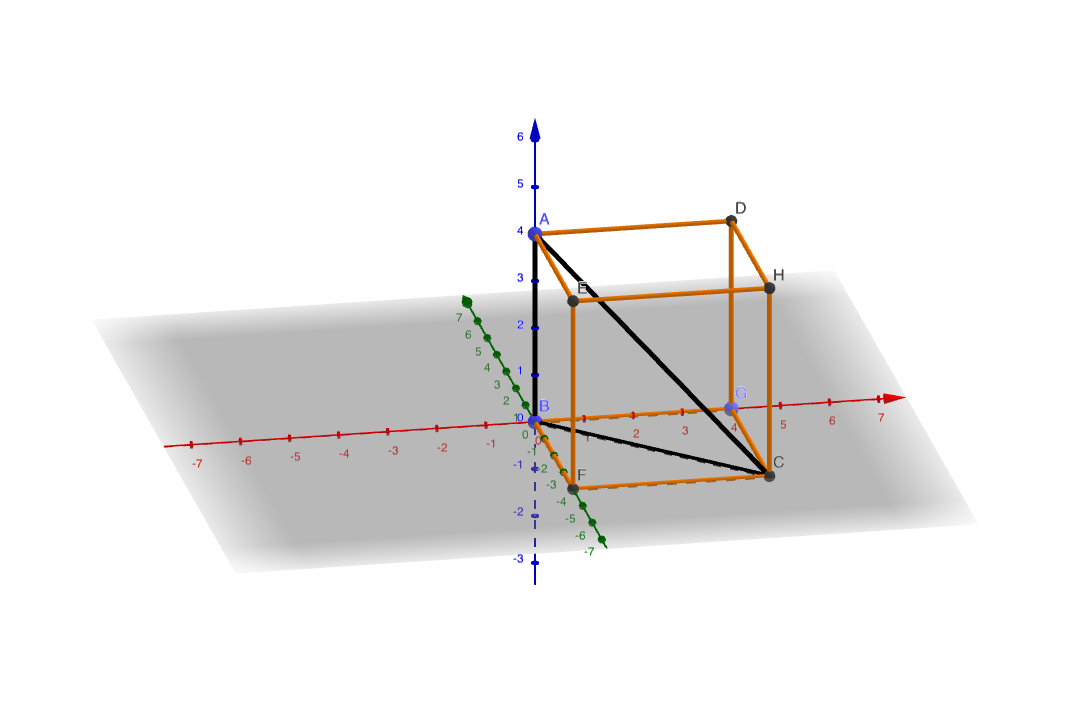
\includegraphics[width=.9\linewidth]{./img/cube-sqrt3-png.png}
\end{center}
\item Montrons par l'absurde que \(\sqrt{3}\) est irrationnel. Soit \(a\)
et \(b\) deux entiers tels que \(\sqrt{3} = \frac{a}{b}\) et
\(pgcd(a, b) = 1\). Alors \(a^2 = 3b^2\). Puisque \(a\) et \(b\) n'ont
pas de diviseur commun il en va de même pour leurs carrés. Donc
3 est un diviseur de \(a\) puisqu'il divise son carré. Ainsi \(a =
       3k\) avec \(k\in\Z\). On peut alors établir que \(a^2 =
       9k^2\) ce qui implique \(b^2 = 3k^2\). Comme \(a^2\) et \(b^2\) n'ont
pas de diviseur commun alors \(k^2\) ne divise pas \(b^2\) donc
nécessairement c'est 3. Problème, si 3 divise \(b^2\) alors il
divise aussi \(b\) ce qui contredit \(pgcd(a, b) = 1\). CQFD
\end{enumerate}

\section{Solution de l'exercice \ref{sec:org73038fa}}
\label{sec:org77e137f}
Voir énoncé \ref{sec:org73038fa}

\begin{enumerate}
\item Le nombre 4 divise le carré de 10 mais pas 10. Le nombre 8
divise le carré de 4 mais pas 4. Le nombre 12 divise le carré
de 6 mais pas 6. Le nombre 16 divise le carré de 8 mais
pas 8. Le nombre 9 divise le carré de 12 mais pas 12.
\item Supposons par l'absurde que le nombre d'or \(\Phi = \frac{1 +
       \sqrt{5}}{2}\) soit rationnel. Alors \(\Phi = \frac{a}{b}\) avec
\(pgcd(a, b) = 1\). Or \(\Phi^2 = 1 + \Phi\) donc \(\Phi^2 =
       \frac{a + b}{b}\in\Q\) mais alors \(\frac{a + b}{b} =
       \frac{a^2}{b^2}\) conduit à \(ab + b^2 = a\) soit \(b^2 = a(b+1)\)
ce qui est absurde car \(a\) ne divise pas \(b\) donc pas son carré
non plus et d'autre par \(b + 1\) ne divise pas \(b^2\) non plus. CQFD
\end{enumerate}
\stopcontents[level-2]
\stopcontents[level-1]

\part{Solutions des exercices de la section : \ref{sec:org7810a4f}}
\label{sec:org1980f56}
\startcontents[level-1]
\printcontents[level-1]{}{0}{\setcounter{tocdepth}{2}}
\begin{foreigndisplayquote}{english}
You don’t have to be a mathematician to have a feel for numbers.\\

\href{https://en.wikipedia.org/wiki/John\_Forbes\_Nash\_Jr.}{John Forbes Nash Jr.}
\end{foreigndisplayquote}

\chapter{Solutions des exercices de la section : \ref{sec:org2051646}}
\label{sec:org448c6a2}
\startcontents[level-2]
\printcontents[level-2]{}{0}{\setcounter{tocdepth}{4}}

\begin{foreigndisplayquote}{english}
It is impossible to be a mathematician without being a poet in soul.\\

\href{https://en.wikipedia.org/wiki/Sofya\_Kovalevskaya}{Sofya Kovalveskaya}
\end{foreigndisplayquote}

\section{Solution de l'exercice \ref{sec:orgc3f82e5}}
\label{sec:orgefbdf8f}
\begin{verbatim}
# Solution
import matplotlib.pyplot as plt
import numpy as np

numbers = [-2, -0.5, 0, 1, np.sqrt(2), np.pi]
labels = ['P_0 (-2)', 'P_1 (-0.5)', 'P_2 (0)', 'P_3 (1)', 'P_4 (√2)', 'P_5 (π)']

plt.figure(figsize=(10, 1))

# Ploter une ligne horizontale
plt.plot([min(numbers), max(numbers)], [0, 0], 'k')

# Placer les nombres sur la ligne graduée
plt.scatter(numbers, np.zeros_like(numbers), color='red')

# Ajouter des étiquettes aux nombres
for i, label in enumerate(labels):
    plt.text(numbers[i], 0.02, label, ha='center')

# Masquer les axes
plt.axis('off')

plt.show()
\end{verbatim}
\stopcontents[level-2]

\chapter{Solutions des exercices de la section : \ref{sec:orge169269}}
\label{sec:orgccc811d}
\startcontents[level-2]
\printcontents[level-2]{}{0}{\setcounter{tocdepth}{4}}

\begin{foreigndisplayquote}{english}
A mathematician who is not also something of a poet will never be a
complete mathematician.\\

\href{https://en.wikipedia.org/wiki/Karl\_Weierstrass}{Karl Weierstrass}
\end{foreigndisplayquote}

\section{Solution de l'exercice \ref{sec:org837f3c6}}
\label{sec:org814b848}
Voir énoncé \ref{sec:org837f3c6}

Pour rappels tous les codes sont accessibles sur Google Colab à
l'adresse communiquée dans la section concernée lorsque vous
aurez rempli ce petit formulaire :
\url{https://forms.gle/pT3GVr8PdNYCeVir7} (vous trouverez également
les corrections de tous les exercices du livre).

C'est également sur Google Colab que vous pourrez tester tous les
programmes qui vous permettent de pratiquer les capacités attendues
de manière interactive.

Voici le code pour générer les solutions de l'exercice \ref{sec:org837f3c6} :
\begin{verbatim}
# Solution
from math import floor, ceil


def default(number, decimals):
  """
  Cette fonction prend 2 paramètres en entrées :
  number: le nombre dont on cherche à faire l'arrondi par défaut
  decimals: le nombre de chiffres après la virgule
  Elle renvoie le nombre arrondi par défaut à decimals décimales
  """
  num = floor(number * 10**decimals)
  den = 10**decimals
  return num / den

def excess(number, decimals):
  """
  Cette fonction prend 2 paramètres en entrées :
  number: le nombre dont on cherche à faire l'arrondi par excès
  decimals: le nombre de chiffres après la virgule
  Elle renvoie le nombre arrondi par excès à decimals décimales
  """
  if number == int(number):
    num = ceil(number * 10**decimals + 1)
  else: num = ceil(number * 10**decimals)
  den = 10**decimals
  return num / den

def get_boundary(nums, method, decimals):
  """
  Cette fonction prend 3 paramètres en entrées :
  nums: la liste de nombres dont on cherche la borne (inf ou sup)
  method: la fonction utilisée (default ou excess)
  decimals: le nombre de décimales
  Elle renvoie la liste des bornes (que des infs ou que des sups)
  """
  bounds = [method(num, decimals) for num in nums]
  return bounds


num_to_square = [1 + i/10 for i in range(5)]
squares = [round(n2s**2, 2) for n2s in num_to_square]
infs = get_boundary(squares, default, 1)
sups = get_boundary(squares, excess, 1)
list_of_intervals = [[infs[i], sups[i]] for i in range(len(infs))]

nums = []
for i in range(len(squares)):
  nums.extend([infs[i], squares[i], sups[i]])
  n2s, interval = num_to_square[i], list_of_intervals[i]
  msg = f"{n2s}**2 = {squares[i]} appartient à l'intervalle {interval}"
  print(msg)

plt.figure(figsize=(10, 1))

# Tracer une ligne horizontale
plt.plot([min(nums), max(nums)], [0, 0], 'k')

# Placer les nombres sur la ligne graduée
plt.scatter(squares, np.zeros_like(squares), color='green', marker='x')
plt.scatter(infs, np.zeros_like(infs), color='red', marker='$[$')
plt.scatter(sups, np.zeros_like(sups), color='red', marker='$]$')

infs_labels = [str(inf) for inf in infs]
sqrs_labels = [str(sqr) for sqr in squares]
sups_labels = [str(sup) for sup in sups]
# Ajouter des étiquettes aux nombres
for i, inf_label in enumerate(infs_labels):
    plt.text(infs[i], 0.02, inf_label, ha='center')

for i, sqr_label in enumerate(sqrs_labels):
    plt.text(squares[i], -0.02, sqr_label, ha='center', va='top')

for i, sup_label in enumerate(sups_labels):
    plt.text(sups[i], 0.02, sup_label, ha='center')


# Masquer les axes
plt.axis('off')

plt.show()
\end{verbatim}
\stopcontents[level-2]

\chapter{Solutions des exercices de la section : \ref{sec:orga688303}}
\label{sec:org632b46d}
\startcontents[level-2]
\printcontents[level-2]{}{0}{\setcounter{tocdepth}{4}}

\begin{foreigndisplayquote}{english}
In mathematics the art of proposing a question must be held of
higher value than solving it.\\

\href{https://en.wikipedia.org/wiki/Georg\_Cantor}{Georg Cantor}
\end{foreigndisplayquote}

\section{Solution de l'exercice \ref{sec:orgba6b593}}
\label{sec:org3cfb91a}
Voir énoncé \ref{sec:orgba6b593}

Les solutions sont générées automatiquement après la saisie
utilisateur.

Pour rappels tous les codes sont accessibles sur Google Colab à
l'adresse communiquée dans la section concernée lorsque vous
aurez rempli ce petit formulaire :
\url{https://forms.gle/pT3GVr8PdNYCeVir7} (vous trouverez également
les corrections de tous les exercices du livre).

C'est également sur Google Colab que vous pourrez tester tous les
programmes qui vous permettent de pratiquer les capacités attendues
de manière interactive.

\section{Solution de l'exercice \ref{sec:org0e68f9c}}
\label{sec:org7cc2be4}
Voir énoncé \ref{sec:org0e68f9c}

Les solutions sont générées automatiquement après la saisie
utilisateur.

Pour rappels tous les codes sont accessibles sur Google Colab à
l'adresse communiquée dans la section concernée lorsque vous
aurez rempli ce petit formulaire :
\url{https://forms.gle/pT3GVr8PdNYCeVir7} (vous trouverez également
les corrections de tous les exercices du livre).

C'est également sur Google Colab que vous pourrez tester tous les
programmes qui vous permettent de pratiquer les capacités attendues
de manière interactive.
\stopcontents[level-2]

\chapter{Solutions des exercices de la section : \ref{sec:orge07749d}}
\label{sec:orgd5714cf}
\startcontents[level-2]
\printcontents[level-2]{}{0}{\setcounter{tocdepth}{4}}

\begin{foreigndisplayquote}{english}
It is clear that the chief end of mathematical study must be to
make the students think.\\

\href{https://en.wikipedia.org/wiki/John\_Wesley\_Young}{John Wesley Young}
\end{foreigndisplayquote}

\section{Solution de l'exercice \ref{sec:org329206f}}
\label{sec:orgfa9b7da}
Voir énoncé \ref{sec:org329206f}

Pour rappels tous les codes sont accessibles sur Google Colab à
l'adresse communiquée dans la section concernée lorsque vous
aurez rempli ce petit formulaire :
\url{https://forms.gle/pT3GVr8PdNYCeVir7} (vous trouverez également
les corrections de tous les exercices du livre).

C'est également sur Google Colab que vous pourrez tester tous les
programmes qui vous permettent de pratiquer les capacités attendues
de manière interactive.

Voici le code pour générer l'exercice :
\begin{verbatim}
# Solution
print(f"Puisque 1 mile = {mile} alors cela fait {mile/1000} km")
print(f"Ainsi 1 km = {1000/mile} miles")
print(f"Il suffit donc de multiplier la vitesse en km/h par {1000/mile}")
a *= 1000/mile
if a > 10:
  a /= 10
  k -= 1
elif a < 1:
  a *= 10
  k += 1
print(f"D'où c = {a} x 10**{k} mph")
\end{verbatim}
\stopcontents[level-2]
\stopcontents[level-1]
\end{document}